% book example for classicthesis.sty
\documentclass[
  % Replace twoside with oneside if you are printing your thesis on a single side
  % of the paper, or for viewing on screen.
  %oneside,
  twoside,
  %openleft,
  %titlepage,
  11pt, letterpaper,
  footinclude=true,
  headinclude=true,
  cleardoublepage=empty
]{book}

\usepackage{lipsum}
%\usepackage[linedheaders,parts,pdfspacing]{classicthesis}
\usepackage{amsmath}
\usepackage{amstext}
\usepackage{amsthm}
\usepackage{acronym}
\usepackage{cite} % para contraer referencias
\usepackage[utf8]{inputenc}
\usepackage[spanish]{babel}
\usepackage{graphicx}
\usepackage[bookmarks=true]{hyperref}
\usepackage{bookmark}
%\usepackage{pdfpages}
\usepackage{float}
\setlength{\parskip}{3mm}
\usepackage{marginnote}



\title{Una propuesta de arquitectura empresarial para valoración colectiva de empresas, productos y servicios usando la especificación Archimate 2.0. y Business Canvas Model}

\author{Ing. Julian Olarte Ramos}

\begin{document}

\maketitle

\graphicspath{{images/}}

%*******************************************************
% Abstract
%*******************************************************
\pdfbookmark[1]{Abstract}{Abstract}
\chapter*{Resumen}

Se propone un modelo de negocio de valoración distribuida y colaborativa de marca (empresas, productos y servicios) a través de una aplicación móvil mostrando una arquitectura basada en cloud y microservicios en cuatro elementos fundamentales: motivaciones e interesados, negocio, aplicación e infraestructura. La propuesta se construye sobre la especificación de descripción arquitectónica Archimate 2.0. y es alimentada usando una descripción ontológica basada en Business Canvas Model.
%*******************************************************
% Dedication
%*******************************************************
\thispagestyle{empty}
\pdfbookmark[1]{Dedication}{Dedication}

\vspace*{3cm}

\begin{center}
    A todos aquellos que se alejan de lo que más quieren para poder apreciarlo desde la distancia.   
\end{center}

%*******************************************************
% Acknowledgments
%*******************************************************
\pdfbookmark[1]{Acknowledgements}{acknowledgements}
\chapter*{Agradecimientos}

Se agradece infinitamente a todos aquellos que aporten a ésta propuesta con sus críticas, ideas, elementos materiales o grandemente con la energía que pueda entregar. 
%*******************************************************
% Table of Contents
%*******************************************************
\pdfbookmark[1]{\contentsname}{tableofcontents}

\setcounter{tocdepth}{2} % <-- 2 includes up to subsections in the ToC
\setcounter{secnumdepth}{3} % <-- 3 numbers up to subsubsections

\tableofcontents

%*******************************************************
% List of Figures and of the Tables
%*******************************************************

%*******************************************************
% List of Figures
%*******************************************************    
\pdfbookmark[1]{\listfigurename}{lof}
\listoffigures

%*******************************************************
% List of Tables
%*******************************************************
%\pdfbookmark[1]{\listtablename}{lot}
%\listoftables
  
%*******************************************************
% List of Listings
%******************************************************* 
%\pdfbookmark[1]{\lstlistlistingname}{lol}
%\lstlistoflistings 
   
%*******************************************************
% Acronyms
%*******************************************************
%\pdfbookmark[1]{Acronyms}{acronyms}
%\chapter*{Acronyms}
%\begin{acronym}[UML]
%    \acro{DRY}{Don't Repeat Yourself}
%    \acro{API}{Application Programming Interface}
%    \acro{UML}{Unified Modeling Language}
%\end{acronym} 


\part{Inicio}
%*******************************************************
% Capitulo uno
%*******************************************************

\chapter{Introducción}

Este documento expone la propuesta de creación de un modelo de negocio basado en una aplicación móvil de valoración y comparación de marcas. El documento está construido usando la especificación Archimate 2.0 \cite{iacob2012archimate} y el Modelo Canvas \cite{osterwalder2013business}\cite{osterwalder2004business}. En el presente capítulo se detallan elementos básicos como el resumen de la propuesta, los referentes que dan origen a la idea y el alcance del documento.

\section{Propuesta}

Se propone un modelo de valoración independiente y colectivo de marcas por medio de una aplicación móvil de descarga gratuita, que además permite retroalimentar a la marca acerca de situaciones específicas sobre atención, calidad de producto o situaciones anormales. Además la aplicación explorará las redes sociales para analizar y publicar información relevante a las marcas.

Dado que cada marca puede representar elementos valorables diferentes como empresas, productos y servicios, se propone la calificación de elementos de manera independiente. Cada administrador de marca podrá controlar qué elementos podrán ser expuestos al consumidor con el fin de organizar los elementos disponibles, de tal manera que cada empresa podrá proponer modificaciones a la base de datos para reunir o especificar sus productos/servicios o definir métricas diferentes a la estándar. Se propone el uso de una base de datos inicial de marcas públicas y privadas.

El modelo de negocio se basa en ads de publicidad para el usuario final, suscripción premium para las empresas en la aplicación y en servicios conexos para empresas que pertenezcan a la base de datos. Entre los servicios ofrecidos pueden estar: Estudios de mercado, publicidad, reestructuración de procesos de atención y servicio al cliente basados en modelos digitales o comunicación online con el cliente.

\section{Antecedentes y referentes}

\subsection{Ejercicio de comparación: Apps de taxis}

El primer referente para la concepción de ésta idea de negocio es la comparación de atributos competitivos en apps de solicitud de taxi en Colombia. Un rápido repaso por cada una de las aplicaciones disponibles en el mercado muestra que UBER \cite{avalos2015baby} vence en diferentes aspectos a otras aplicaciones resaltando un atributo en particular: la calificación al conductor. 

Los esquemas de valoración tienen efectos de control y aseguramiento de la calidad porque permiten tomar acciones sobre los prestadores. Los mismos efectos de valoración se pueden ver en organizaciones que han implementado medidas de valoración que transforman calificaciones en medidas de tracción de usuarios. En el caso de Uber los conductores valorados por debajo de 4.0 reciben sanciones que impiden que se vuelvan a presentar futuros inconvenientes, ya sea porque se corrige el comportamiento del conductor o se retira de la plataforma.

\subsection{Aplicaciones de valoración de nicho específico}

El segundo referente importante son las aplicaciones de valoración de servicios en nichos específicos. Por ejemplo, en el sector del turismo y similares se encuentran aplicaciones con diferentes alcances como \textit{tripadvisor} o \textit{foursquare}. Cada una de ellas comparte el mismo modelo encontrado en el primer referente: la valoración por el usuario para la marca. En el sector educativo se pueden encontrar aplicaciones como SchoolMars, cuyo epígrafe es \textit{"Ponle nota a tu colegio"}\cite{schollmars:2013:Online}. 
Para cada nicho de mercado se pueden encontrar aplicaciones, unas más populares que otras, que permiten construir conocimiento colectivo de valoración empresarial de productos o servicios.

En latinoamérica existen los siguientes referentes que pueden ser consultados: \textit{http://www.apontador.com.br/} lider en Brasil en la valoración de lugares de entretenimiento y \textit{https://kekanto.com.co/} También una empresa brasilera pero con presencia en Colombia, y \textit{http://www.guiatodo.com.co/} empresa colombiana que reúne información de sitios de turismo.

\subsection{Redes sociales}

El tercer referente es el uso de las redes sociales como canal de expresión de las valoraciones y percepciones de marca. Todos los días Twitter, Facebook, Instagram, Snapchat, son usadas por usuarios para manifestar inconformidad con algún producto o servicio. La información publicada  reemplaza al tradicional voz a voz y con quejas de alto tono se logra difusión viral de la molestia. 

Las marcas han tenido que enfrentar los nuevos canales mediante community managers y otros cargos que antes no existían. La estrategia actual es hacer contrapeso a las publicaciones con impactos positivos de marca y disuación de comentarios. Aunque ésta información es muy relevante se pierde en el flujo natural de las redes y en cuestión de horas son publicaciones del pasado. Es importante notar que en este momento no se está capitalizando la información distribuida en las redes sociales.

\subsection{Aplicaciones de valoración global}

Los referentes más cercanos a la presente idea de negocio son \textit{Google Reviews} y \textit{yelp.com}\cite{luca2011reviews}. Google Reviews es una plataforma que permite a los usuarios realizar reseñas para locales comerciales o empresas con el fin de entregar a los próximos usuarios una valoración que es útil para tomar decisiones basadas en información construida por los usuarios de las marcas que también usan Google. 

\textit{Yelp.com} es un sitio web y aplicación movíl donde los consumidores pueden dejar revisiones y comentarios de restaurantes y otros comercios. Fue fundada en 2004, en San Francisco. Para el año 2011 contenían más de 10 millones de revisiones y recibía mas de 40 millones de visitantes únicos por mes en estados unidos. Actualmente no tienen presencia en los países de suramérica.

\section{Alcance y limitaciones}

Este documento presenta una descripción arquitectónica por medio de los puntos de vista de la especificación Archimate 2.0. incluyendo capa motivacional, negocio, aplicación e infraestructura. No se describe ningún aspecto de la viabilidad financiera. Para la descripción arquitectónica se usa una construcción básica del negocio obtenida a partir del modelo canvas. 

Las siguientes partes del documento describen aspectos básicos de la metodología y el lenguaje usado en el documento, la información obtenida después del análisis bajo la propuesta Business Canvas Model\cite{osterwalder2004business} y en la tercera parte del documento cada una de los puntos de vista de Archimate 2.0. Al final algunas conclusiones y trabajo futuro para mejorar ésta presentación. 

%*******************************************************
% Capitulo dos ///// SE Modifica para el capitulo uno
%*******************************************************

\section{Metodología}

El proceso de especificación del modelo de negocio tiene tres etapas principales:
\begin{itemize}
    \item Recolección de referentes fundamentales y examen de la competencia (documentado en el Capítulo 1).
    \item Análisis de modelo de negocio con la estructura Business Canvas Model \cite{osterwalder2004business} y descripción de los nueve cuadrantes.
    \item Descripción avanzada de la propuesta usando los 15 puntos de vista de la especificación Archimate 2.0.
\end{itemize}

El proceso de construcción pasa por la especificación de cuatro capas, a saber: Capa Motivacional, capa de negocio, capa de aplicación y capa de infraestructura.


%*******************************************************
% Capitulo dos
%*******************************************************

\chapter{Lenguaje usado}

La descripción de los componentes de arquitectura empresarial y sus relaciones requieren un lenguaje de modelado que guíe de manera elocuente la exposición de todos los detalles del negocio.

Éste documento usa la especificación de modelado arquitectónico ArchiMate 2.0. \cite{iacob2012archimate} para facilitar la exposición de la presente propuesta. El diseño del lenguaje ArchiMate inicia desde un conjunto de conceptos genéricos como entidad y relación y agrega a especificaciones anteriores, como UML, una gran variedad de conceptos específicos que derivan de procesos y aplicaciones de procesos para después aplicar conceptos específicos de dominio y arquitectura empresarial. 

A continuación se expone brevemente los detalles más importantes del estándar de modelado.

\section{Conceptos principales}

Los tres elementos principales del lenguaje, que representan entidades del mundo real, son: Elementos estructurales activos, Elementos de comportamiento y Sujetos que expresan dicho comportamiento o en otras palabras objetos.

\begin{itemize}
    \item Un \textit{elemento estructural activo} es definido como una entidad capaz de ejecutar un comportamiento.
    \item Un \textit{elemento de comportamiento} es una unidad ejecutada por uno o más elementos estructurales activos.
    \item Los \textit{elementos estructurales pasivos} son objetos en los que un comportamiento es ejecutado.
\end{itemize}

Éstos tres aspectos son inspirados en frases con sujetos (estructuras activas), verbos (comportamientos) y objetos (estructuras pasivas).

Por otro lado, se realiza una distinción entre la vista interna y externa de un sistema y estas se conectan. Bajo esta conexión se aclara también el termino de interfaz.

\begin{itemize}
    \item Un \textit{servicio} es una unidad de funcionalidad expone un sistema a su ambiente mientras oculta operaciones internas que entregan valor.
\end{itemize}

Dado que el servicio es el comportamiento visible externo de un sistema, existe un entorno en el que el sistema es usado a través del servicio. El servicio existe por una motivación que debe ser entendida como el valor del sistema o el servicio. Para los que usan de manera externa la combinación del servicio y su valor sólo no es relevante la información interna del sistema. Los servicios son accequibles a través de interfaces, las cuales son la vista externa de un elemento activo.

\begin{itemize}
    \item Una \textit{interfaz} es definida como un punto de acceso para uno o más servicios y esta disponible al entorno del sistema.
\end{itemize}

\section{Colaboración e interacción}

En ArchiMate se puede distinguir entre un comportamiento realizado por un elemento estructural o un comportamiento colectivo (interacción) que es ejecutado por una colaboración de múltiples elementos estructurales.

\begin{itemize}
    \item Una \textit{colaboración} es definida como una agrupación de dos o más elementos estructurales que desarrollan un comportamiento colectivo.
\end{itemize}

El comportamiento colectivo puede ser modelado como una interacción.

\begin{itemize}
    \item Una \textit{interacción} es definida como una unidad de comportamiento ejecutada por una colaboración de dos o más elementos estructurales.
\end{itemize}

\section{Relaciones y capas}

Para relacionar las entidades, ArchiMate cuenta con una serie de relaciones análogas a otros lenguajes gráficos de modelado como UML o BPMN.

También cuenta con tres capas principales basadas en especializaciones de los conceptos básicos. 

\begin{enumerate}

\item La capa de negocio ofrece productos y servicios a clientes  externos, los cuales son realizados en la organización por procesos de negocio y actores del negocio.

\item La capa de aplicación soporta el negocio con servicios de aplicación que son realizados por aplicaciones (software).

\item La capa de tecnología (Infraestructura) ofrece servicios de infraestructura (por ejemplo: procesamiento, almacenamiento y servicios de comunicación) usados para ejecutar aplicaciones realizadas por computadores, hardware de comunicación y sistemas de software.

\end{enumerate}




%*******************************************************
% Capitulo tres
%*******************************************************

\chapter{Modelo Canvas}

La propuesta para describir modelos de negocio presentada por Osterwalder en \cite{osterwalder2004business} muestra un esquema en donde nueve módulos básicos reflejan la lógica que sigue una empresa para conseguir ingresos. Estos nueve módulos cubren las cuatro áreas principales de un negocio: clientes, oferta, infraestructuras y viabilidad económica.

El Modelo Canvas describe una composición de modelo de negocio donde la propuesta de valor (que hace parte del producto junto con la oferta) ocupa una posición central. Esta tiene que ser llevada a unos segmentos de clientes con los que se establecerán unas relaciones. Para hacerlo hay que describir unos canales específicos. Internamente, se deben desarrollar unas actividades clave con unos recursos clave. Para lograrlo se interactúa con unos Aliados importantes. 

Finalmente se especifican los elementos que permiten sustentar la operación en términos de costos y las fuentes de ingreso del modelo de negocio.

\section{Aliados clave}

\textbf{¿Quienes son sus aliados clave y proveedores?}

Los aliados clave del negocio se dividen en los diferentes proveedores de tecnología que sustentan la operación y los aliados estratégicos que complementan el portafolio de servicios. Entre ellos se encuentran:

\begin{itemize}
    \item Proveedor para colocación de Ads (publicidad online) de terceros dentro de la aplicación.
    \item Proveedor para colocación de Ads en portales de internet para promocionar la aplicación.
    \item Proveedor de cloud para el despliegue de los servicios.
    \item Aliado de desarrollo de servicios de software.
    \item Aliado de consultoría en servicios de marca y publicidad.
  
\end{itemize}

\section{Actividades clave}

\textbf{¿Cuáles son las actividades más importantes en la ejecución de sus propuestas de valor?}

Las actividades principales describen aspectos de la operación y la gestión comercial. Entre ellos están:

\begin{itemize}
    \item Activación de nuevas cuentas empresariales.
    \item Procesos de servicio y consultoría sobre las cuentas.
    \item Despliegue de aplicaciones.
    \item Innovación y desarrollo en requisitos funcionales de la app.
    \item Gestión de conocimiento y análisis de datos.
    \item Tracción de nuevos usuarios finales.
\end{itemize}   

\section{Recursos clave}

\textbf{¿Cuáles son los recursos clave en la ejecución de las propuestas de valor?}

Dada la naturaleza del negocio, los recursos clave están enfocados tanto en talento humano como en la tecnología que permite la operación. Entre ellos está: 

\begin{itemize}
    \item Los desarrolladores de la aplicación.
    \item Los ambientes de desarrollo de software, pruebas y producción.
    \item La información local y externa acerca de las marcas.
    \item Los consultores en temas de marcas y en temas de atención y servicio al cliente
\end{itemize}   

\section{Propuestas de valor}

\textbf{¿Qué valor se le entregará a los clientes? ¿Qué problemas se les está ayudando a resolver?}

La propuesta de valor es el elemento más importante de la construcción del Modelo Canvas y puede ser entendida como la declaración de los beneficios que son entregados por el negocio. En este caso los externos que reciben éstos beneficios se dividen en dos. 

A la sociedad en general representada en los usuarios de la aplicación se le ofrece,
\begin{itemize}
    \item La oportunidad de tomar decisiones acertadas de relacionamiento frente a una marca basada en experiencias anteriores y sus métricas de cambio.
    \item Un espacio colectivo e independiente para que su voz sea escuchada en eventos relacionados con algún producto servicio o empresa.
\end{itemize}   

Al universo empresarial representado en las marcas con presencia en la aplicación, 
\begin{itemize}
    \item Organizar la información online de percepción de las marcas.
\end{itemize}

\section{Relaciones con los clientes}

\textbf{¿Qué tipo de relaciones con cada uno de los segmentos de clientes se espera establecer y mantener?}

Este elemento describe la relación que el negocio establece con un segmento de clientes. Una relación está basada sobre el valor (adquisición, retención, venta agregada, etc.) del cliente y en describir sus mecanismos de relacionamiento. Las relaciones con los clientes promueven la proposición de valor y son mantenidas con todo un segmento.

Cada uno de los mecanismos inicialmente planteados por los que se cumple el relacionamiento se describe a continuación.

\begin{itemize}
    \item Campaña sobre el concepto de queja con intervención en espacios físicos y espacios digitales de redes sociales. \textit{Adquisición}. \textit{Usuarios finales}.
    \item Campaña de -A mi también me paso- para construcción de voz a voz digital. \textit{Adquisición}. \textit{Usuarios finales}.
    \item Campaña sobre el concepto de calidad de servicio en espacios digitales de redes sociales. \textit{Adquisición}. \textit{Marcas}.
    \item Programa de comunicación frecuente con estadísticas de interés. \textit{Retención}. \textit{Usuarios finales} y \textit{Marcas}.   
    \item Característica funcional de -Pregúntale al usuario- para generar conversación. \textit{Retención}. \textit{Usuarios finales}.
    \item Portal de mejoramiento continuo en atención y servicio. \textit{Venta agregada}. \textit{Marcas}.
    \item \textbf{Aplicación móvil}. Elemento de relación funcional principal. \textit{Retención}. \textit{Usuarios finales}.
    \item \textbf{Portal de administración de marca.} \textit{Venta agregada}. \textit{Marcas}.
    
\end{itemize}

\section{Segmentos de clientes}

\textbf{¿Cuáles son los segmentos de clientes y usuarios?}

Se tendrá relación con dos tipos de clientes diferentes: Los usuarios finales de la aplicación, los cuales la descargarán de las tiendas de app y usarán regularmente en la valoración, que estarán en la clasificación de usuarios del milenio (millenials); y las marcas valoradas a través de la aplicación, las cuales serán empresas cuya percepción de marca pueda ser recolectada de manera digital. Resumiendo:

\begin{itemize}
    \item \textit{Usuarios finales}. En el segmento de los usuarios del milenio. 
    \item \textit{Empresas}. Pueden ser medianas y grandes de cualquier segmento de mercado que usen o estén interesadas en usar relacionamiento digital con sus usuarios.
\end{itemize}

En cualquier momento se podrá clasificar a los usuarios/marcas como activos e inactivos. Si bien se puede lograr adquisición de los clientes y usuarios podría no cumplirse la retención para algunos. Aquellos en los que se sufra abandono se considerarán como inactivos.

\section{Canales}

\textbf{¿Cuáles son las rutas de acceso o canales para acceder a los clientes?}

Indiscutiblemente los medios digitales forman parte de este modelo de negocio. La forma en la que los usuarios llegarán a las tiendas online y descargarán la aplicación dependerá de las estrategias de adquisición de clientes pero el medio importante considerado como canal serán las tiendas. Los clientes que representan las marcas accederán por el \textit{portal de administración de marca} descrito antes y a él llegarán por un website comercial que mostrará los servicios de negocio. En resumen:

\begin{itemize}
    \item \textit{Portal modelo de negocio}. Antes de registrarse, las empresas propietarias de las marcas accederán a un portal de registro y especificación de planes. 
    \item \textit{Portal de administración de marca}. Compra de otros servicios al tener acceso al modelo de administración de información de la marca.
    \item \textit{Alianzas de crecimiento vertical}. Entrar al sistema a partir de una red de portales aliados en donde se pueda hacer crecimiento vertical de clientes con producto de este modelo de negocio.
    \item \textit{Convenios empresariales}. Convenios con organizaciones empresariales como Cámaras de comercio para afiliaciones masivas.
    \item \textit{Marketplaces}. Las tiendas online de descarga de aplicaciones.
\end{itemize}

\section{Estructura de costos}

\textbf{¿Cuáles son sus costos? ¿Cuáles son los costos más altos?}

Para el funcionamiento de la aplicación se requiere una infraestructura escalable que soporte los servicios a los usuarios y marcas con un \textit{ans} más que aceptable. Además, el crecimiento constante de funcionalidades sobre la aplicación exige un grupo de desarrollo de software permanente capaz de responder con rapidez a actualizaciones de sistemas operativos entre otros. La tarea de activar nuevos clientes recae sobre un departamento comercial que constantemente está buscando la manera de traer nuevas marcas. En resumen:

\begin{itemize}
    \item \textit{Infraestura cloud}. Para soportar los servicios de operación. 
    \item \textit{Equipo de desarrollo}. Para el desarrollo permamente del software.
    \item \textit{Operación de mercadeo y comercial}. Para generar el relacionamiento con los clientes.
\end{itemize}

\section{Flujos de ingresos}

\textbf{¿De qué forma de capturarán ingresos a partir de las proposiciones de valor?}

Se capturarán ingresos de varias formas diferentes, a saber: El posicionamiento deseado de ciertas compañías dentro de la aplicación, incluyendo ads y entrega de publicidad; y los servicios agregados hacia las compañías propietarias de marcas que quieran cambiar su percepción de marca. Entre los servicios agregados también existe la posibilidad de construcción de software para atención y servicio al cliente. La aplicación no tendrá costo para los usuarios finales por lo que será de descarga gratuita. Finalmente la estructura de ingresos dependerá de: 

\begin{itemize}
    \item \textit{Niveles de suscripción de empresas dueñas de marcas}. Tener acceso a administrar la información de la marca. 
    \item \textit{Posicionamiento dentro de la aplicación}. Para presentar resultados de búsqueda prioritarios a los usuarios. 
    \item \textit{Servicios agregados de posicionamiento de marca}. Consultoría específica de posicionamiento y cambio de percepción de marca.
    \item \textit{Servicios agregados en atención y servicio al cliente}. Consultoría en procesos y construcción específica de herramientas de prestación de servicio a través o fuera de la aplicación.
    \item \textit{Estudios y datos}. Consultoría y minería en datos específicos de percepción y demografía del consumidor.
\end{itemize}



\part{Arquitectura}
%*******************************************************
% Capitulo cuatro
%*******************************************************

\chapter{Arquitectura empresarial}

El presente diseño toma como insumo la descripción de nueve cuadrantes del Modelo Canvas y extiende los detalles para cada concepto usando la especificación ArchiMate 2.0. Se describen cuatro capas fundamentales: Motivación, Negocio, Aplicación e Infraestructura. La especificación ArchiMate además agrega otro conjunto de elementos conocido como Implementación y migración (o despliegue). 

En cada capa, se usan los diferentes elementos básicos de ArchiMate: las estructuras activas, los comportamientos y las estructuras pasivas. El modelo tiene una correspondencia con el modelo TOGAF \cite{josey2011togaf} en el que cada capa corresponde con un conjunto de los elementos que dirigen la descripción arquitectónica. Como se ve en la figura \ref{togafarchimate}, los esquemas de colores que describen las diferentes capas también describen su composición dentre de TOGAF.

\begin{figure}[h]\label{togafarchimate}
\centering
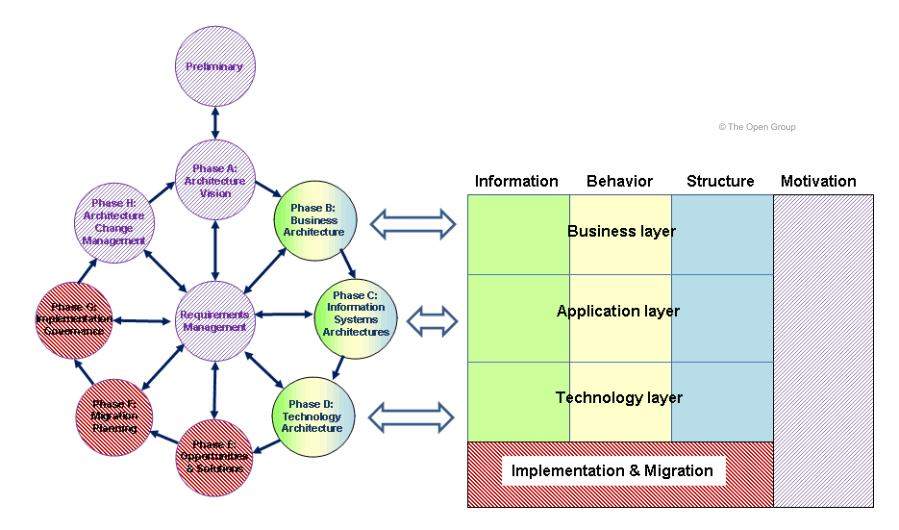
\includegraphics[scale=0.8]{togafarchimate}
\caption{Correspondencia entre Archimate y TOGAF.}
\end{figure}

En los capítulos siguientes se describe cada una de las diferentes capas que permiten la descripción arquitectónica. Cada capa está descrita por diferentes puntos de vista. Cada capitulo contendrá una colección de puntos de vista para cada capa.

Adicionalmente, como notas al margen, se incluirán las ejemplificaciones de los conceptos ArchiMate que heredan de los conceptos básicos. 
%*******************************************************
% Capitulo cinco
%*******************************************************
\chapter{Capa motivacional y de despliegue}

\section{Stakeholders}

\marginpar{\begin{figure}[H]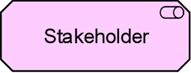
\includegraphics[scale=0.8]{istakeholder}\end{figure} \footnotesize \textbf{Stakeholder}. El rol de un individuo, equipo, o organización (o alguna clase de ellas) que representa sus intereses en, o su relación con, el resultado de la arquitectura.\\}

\marginpar{\begin{figure}[H]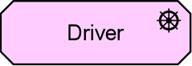
\includegraphics[scale=0.8]{idriver}\end{figure} \footnotesize \textbf{Manejador}. Algo que crea, motiva y alimenta el cambio en la organización.\\}

El punto de vista de los Stakeholders permite modelar las partes interesadas, los manejadores internos y externos, y las evaluaciones (en términos de fortalezas, debilidades, oportunidades y amenazas) de estos manejadores. Además, también modela los vínculos con los objetivos iniciales (de alto nivel) y las valoraciones que puedan ser descritas. Estos objetivos constituyen la base para el proceso de ingeniería de requisitos, incluyendo el refinamiento de los objetivos, análisis de conflictos y contribuciones, y la derivación de los requisitos que realizan los objetivos.

\begin{figure}[H]
\centering
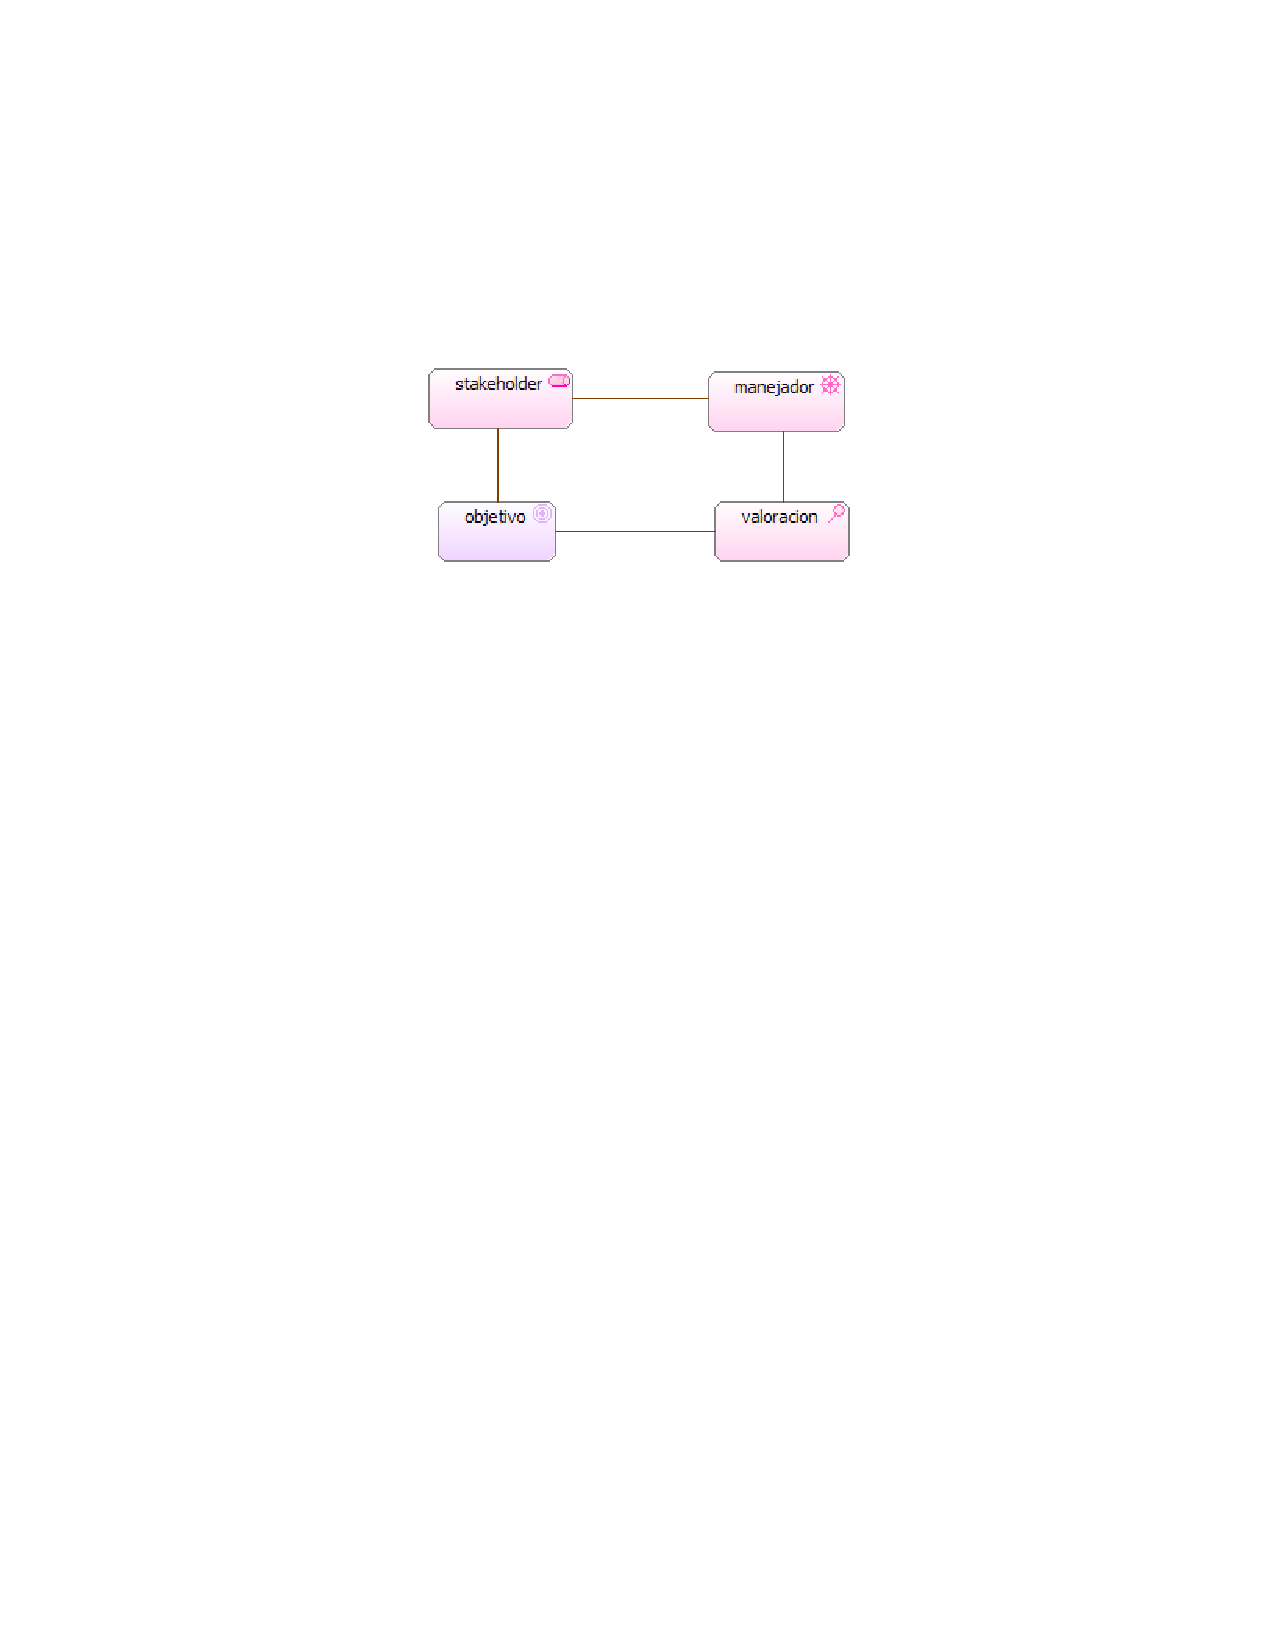
\includegraphics{stakeholder}
\caption{Metamodelo del punto de vista de stakeholder.}
\end{figure}

\marginpar{\begin{figure}[H]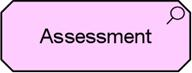
\includegraphics[scale=0.8]{iassessment}\end{figure} \footnotesize \textbf{Valoracion}. El resultado de un análisis de algún manejador.\\}

\marginpar{\begin{figure}[H]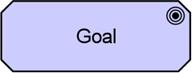
\includegraphics[scale=0.9]{igoal}\end{figure} \footnotesize \textbf{Objetivo}. Un estado final que un stakeholder pretende alcanzar.}

En esta propuesta los Stakeholders externos son los Clientes, Usuario final, Proveedores de servicios de TI, Proveedores de servicios de ads, Consultores y Socios de negocios. Los Stakeholders internos son Gestores de conocimiento, Directores de producto y Directores de cuenta. Algunos de ellos se relacionan con Manejadores (Drivers) los cuales impulsan los objetivos. Una vista de los Stakeholders principales de este negocio puede verse en la figura \ref{diagramastakeholders}, la cual refleja algunos de los cuadrantes del modelo canvas.

\begin{figure}[H]
\centering
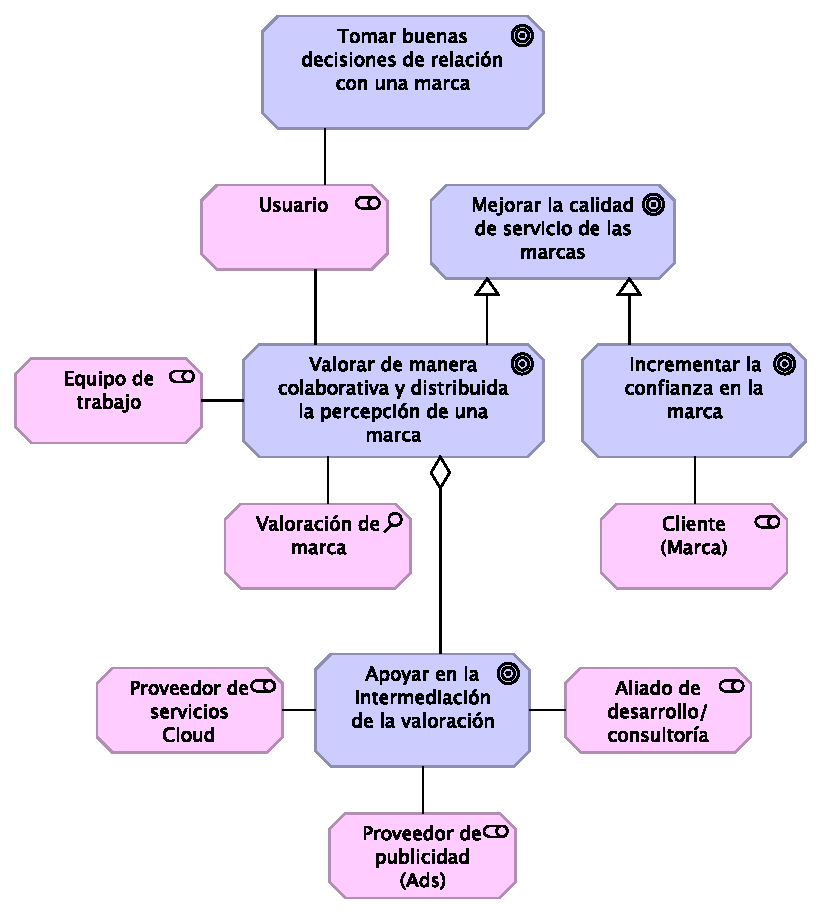
\includegraphics[scale=0.85]{Mstakeholders}
\caption{Punto de vista de stakeholder.}
\label{diagramastakeholders}
\end{figure}

El objetivo es la Mejora de la calidad en el servicio de las marcas. Que se especializa en dos objetivos importantes: Valorar de manera colaborativa y distribuida las marcas e Incrementar la confianza en la marca, este último ejecutado por el equipo de trabajo; y el objetivo de Incrementar la confianza en la marca, ejecutado por el cliente mismo. Otros stakeholders como los proveedores o alidados, descritos en el canvas, apoyan el objetivo de la intermediación en la valoración. 

\section{Realización de objetivos}

El punto de vista de realización de objetivos permite modelar el refinamiento de los objetivos (de alto nivel) en objetivos más concretos, y el refinamiento de objetivos concretos en requisitos o condiciones que describen las propiedades que son necesarias para alcanzar los objetivos. 

El refinamiento de objetivos en sub-objetivos se modela utilizando relaciones de agregación. El refinamiento de las metas en los requerimientos se modela utilizando la relación de realización. Además, los principios pueden ser modelos que guían el refinamiento de los objetivos soportándose con los requisitos.

\begin{figure}[H]
\centering
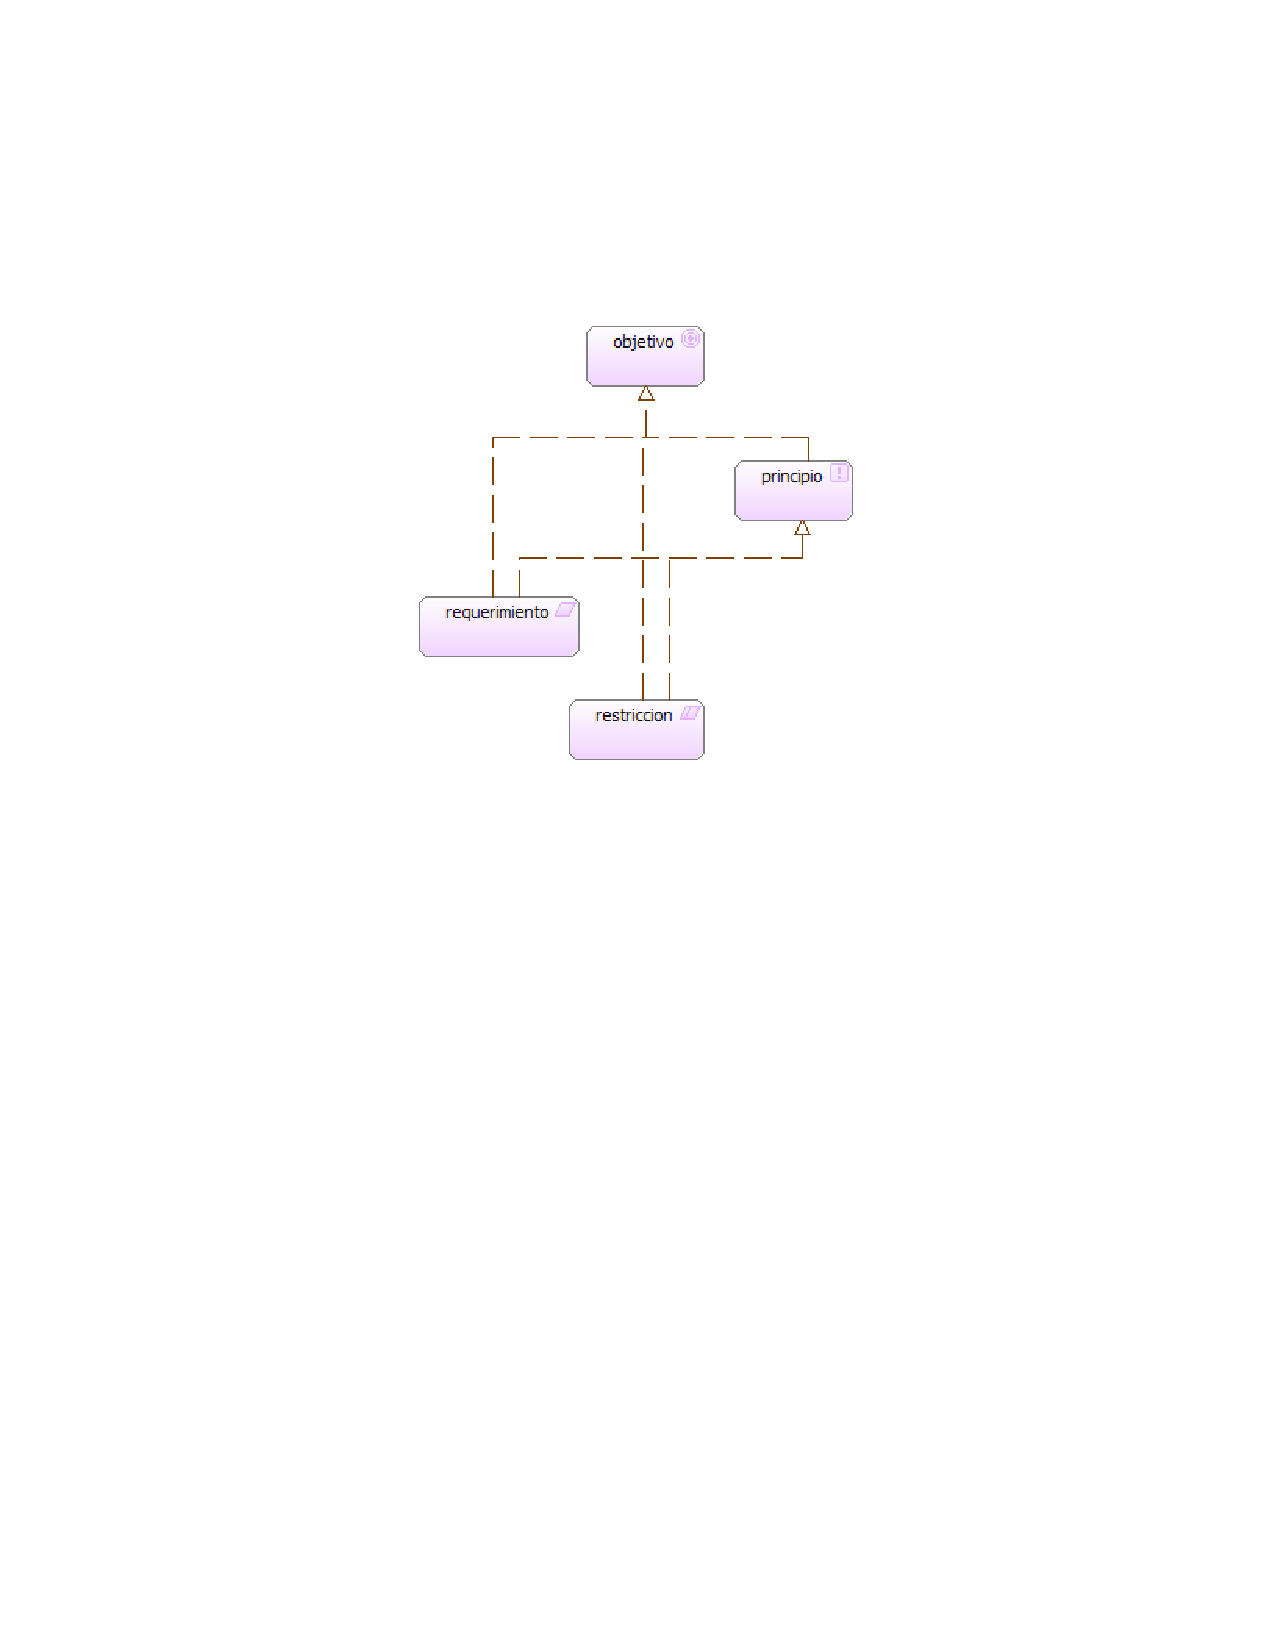
\includegraphics[scale=0.9]{realizacion_de_objetivos}
\caption{Metamodelo del punto de vista de realización de objetivos.}
\end{figure}

\marginpar{\begin{figure}[H]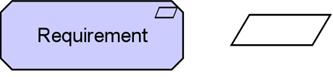
\includegraphics[scale=0.7]{irequeriment}\end{figure} \footnotesize \textbf{Requerimiento}. Una necesidad que debe ser realizada por un sistema.\\}

\marginpar{\begin{figure}[H]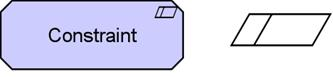
\includegraphics[scale=0.7]{iconstraint}\end{figure} \footnotesize \textbf{Restricción}. Restricción en la forma que un sistema debe ser realizado.}

La realización de objetivos nos muestra algunos de los requisitos más importantes que deben ser creados: la valoración de las marcas, la comparación y la gestión de información de la marca. Una restricción importante es lograr una valoración cuantitativa que permita hacer la comparación.

\begin{figure}[H]
\centering
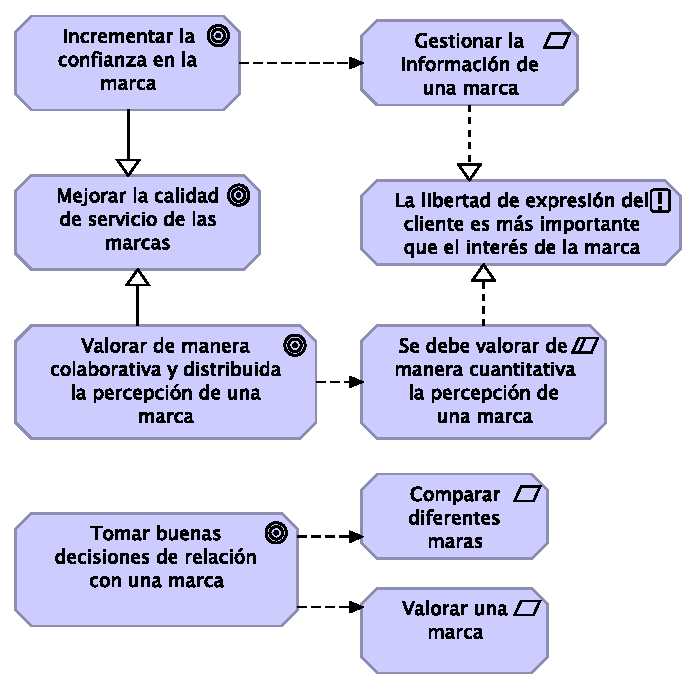
\includegraphics[scale=1]{MRealizaciondeobjetivos}
\caption{Punto de vista de realización de objetivos.}
\end{figure}

\section{Contribución de objetivos}
El punto de vista de contribución de objetivos permite a un diseñador o analista modelar las relaciones que influyen entre los objetivos y requisitos. El resultado de este punto de vista se puede utilizar para analizar el impacto que tienen sobre los objetivos entre sí o para detectar conflictos entre los objetivos de las partes interesadas. Por lo general, este punto de vista se puede utilizar después de  que los objetivos han, en cierta medida, sido refinados en sub-objetivos y, posiblemente, en requisitos. Por lo tanto, las relaciones de agregación y de realización también se puede mostrar en este punto de vista.

\begin{figure}[H]
\centering
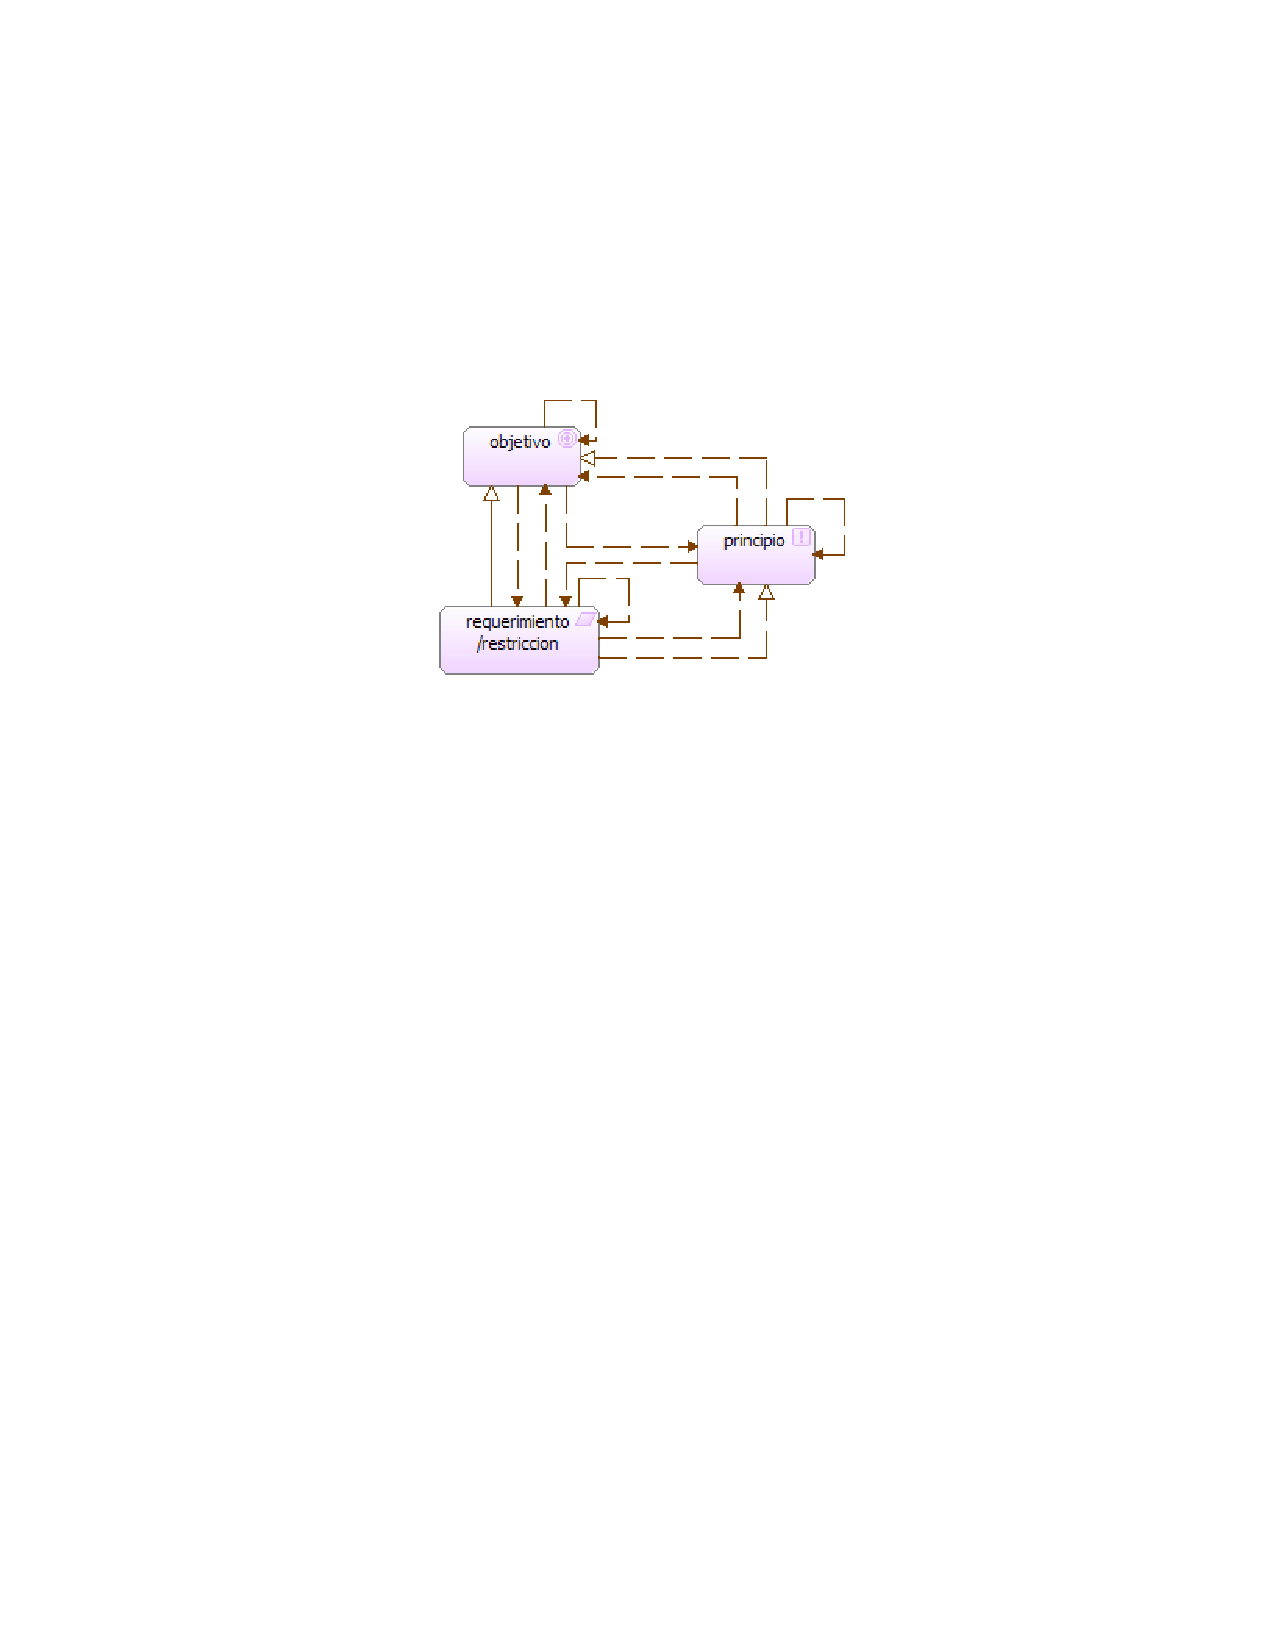
\includegraphics{contribucion}
\caption{Metamodelo del punto de vista de contribución de objetivos.}
\end{figure}

Es de destacar que en la presente propuesta el objetivo de mejorar la calidad de servicio de las marcas es afectado por el requerimiento de comparar diferentes marcas. Esta situación ocurre bajo la consideración que el usuario puede escoger de manera libre el mejor prestador del servicio al poder hacer la comparación. Una vez las marcas entienden que pueden ser escogidas de acuerdo a la percepción difundida y usada para la comparación mejorarían su servicio.

\begin{figure}[H]
\centering
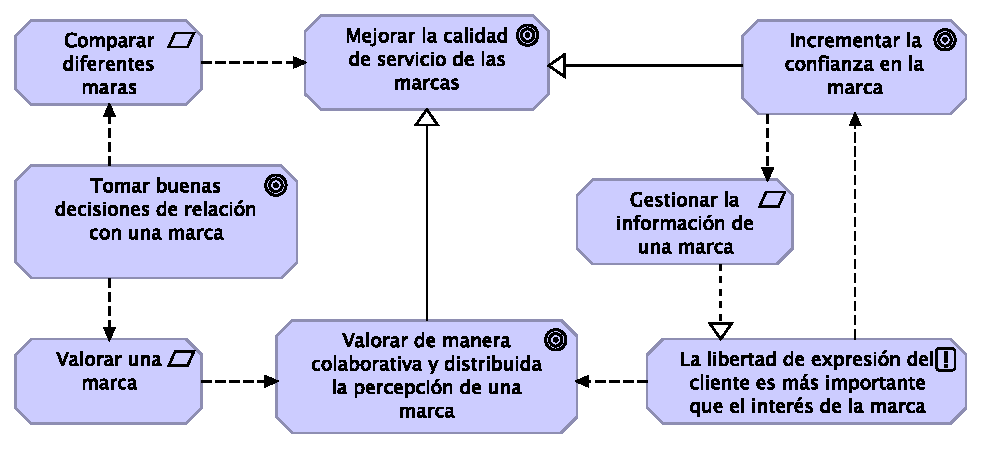
\includegraphics[scale=0.8]{MContribucion}
\caption{Punto de vista de contribución de objetivos.}
\end{figure}

\section{Principios}

\marginpar{
    \begin{figure}[H]
        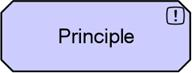
\includegraphics[scale=0.8]{iprinciple}
    \end{figure} 
    \footnotesize 
    \textbf{Principio}. Una propiedad normativa de todos los sistemas en un contexto dado, o la forma en que se realizan.
}

El punto de vista de los principios permite al analista o diseñador modelar los principios que son relevantes para diseñar el problema a mano, incluyendo los objetivos que motivan a estos principios. Además, las relaciones entre los principios y sus objetivos, pueden ser modelados. Por ejemplo, los principios pueden influir entre sí positiva o negativamente.

\begin{figure}[H]
\centering
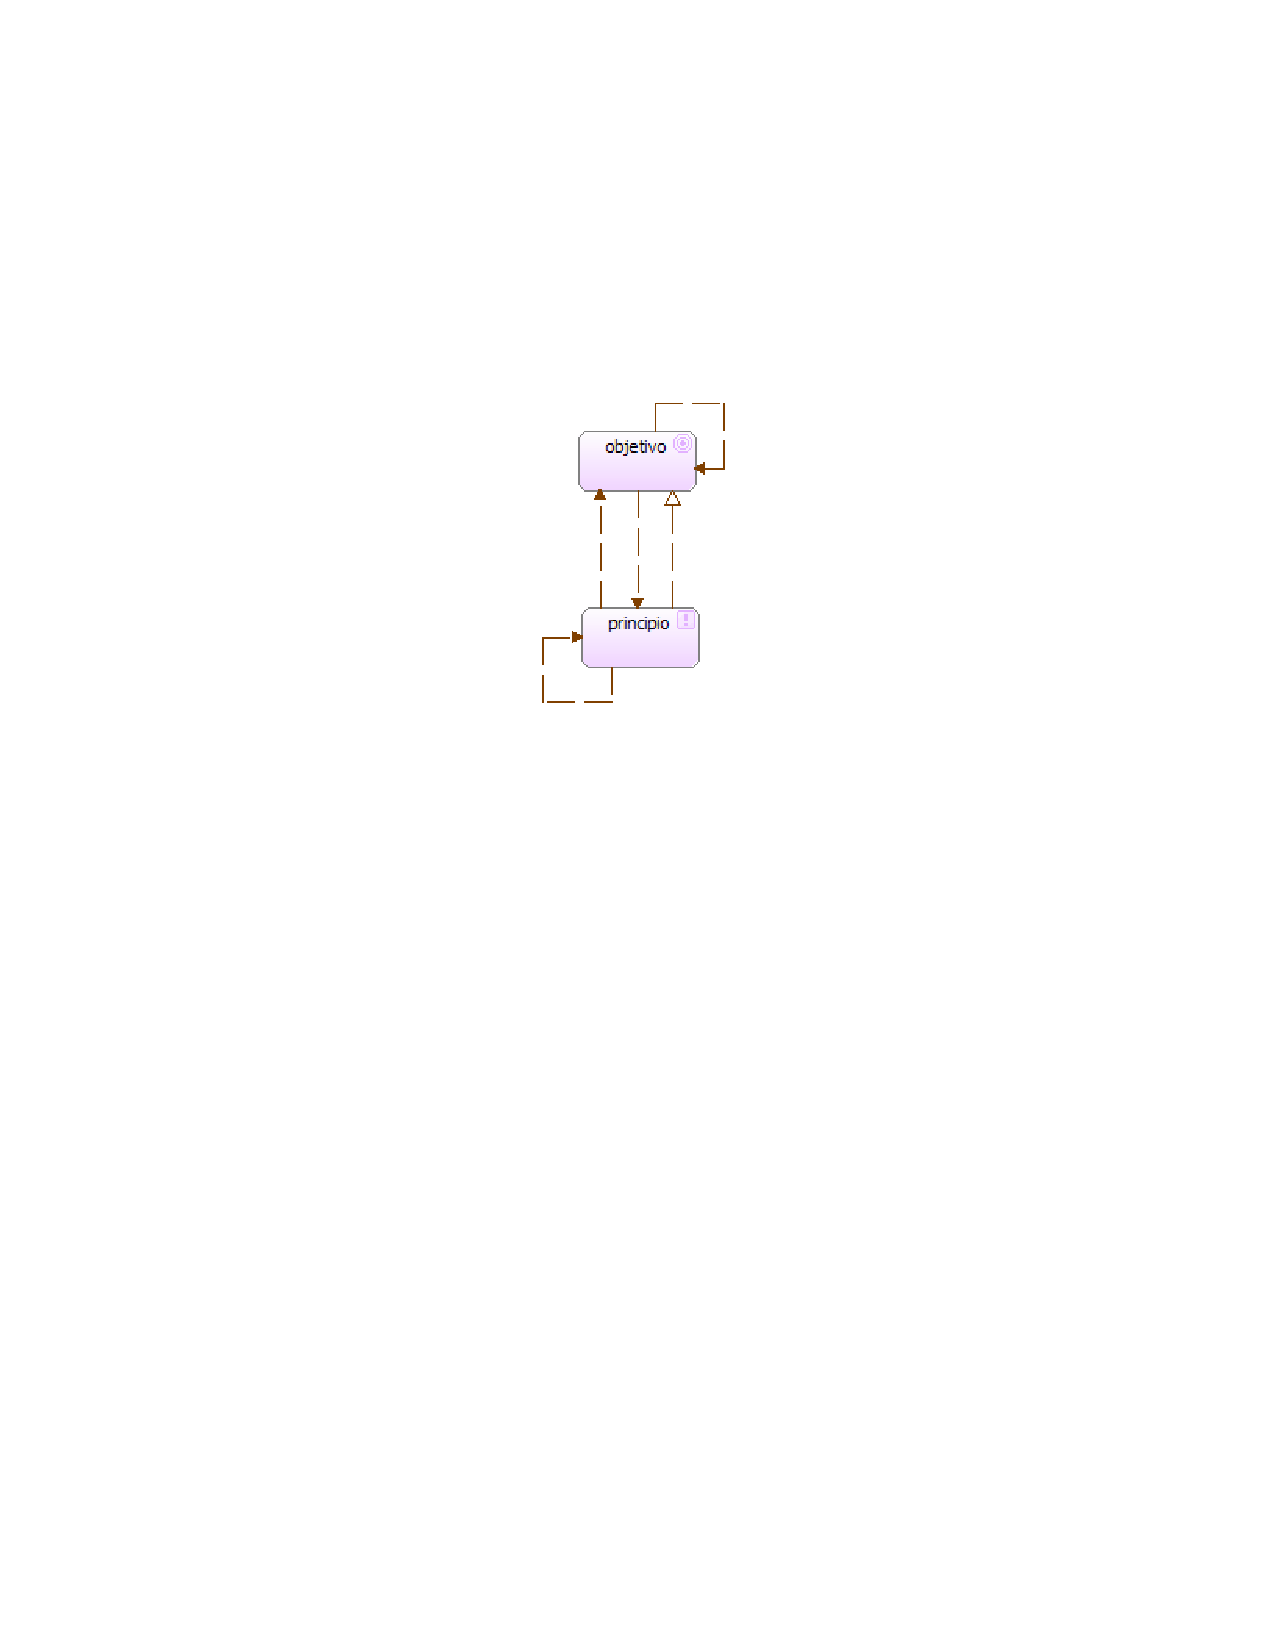
\includegraphics[scale=0.8]{principios}
\caption{Metamodelo del punto de vista de principios.}
\end{figure}

El principio principal es que \textit{La libertad de expresión del cliente es más importante que el interés de la marca}. Tiene un significado muy importante: el diseño de la aplicación es principalmente para beneficiar al usuario con información de calidad sin censura.

\begin{figure}[h]
\centering
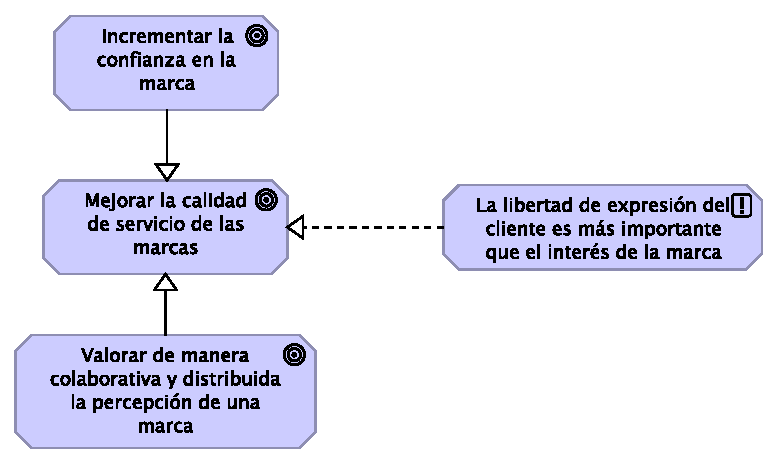
\includegraphics[scale=1]{MPrincipios}
\caption{Punto de vista de principios.}
\end{figure}


\section{Realización de requisitos}

El punto de vista de realización de requisitos permite al diseñador modelar la realización de los requisitos por parte de los elementos básicos, tales como agentes de negocios, servicios de oficina, los procesos de negocios, servicios de aplicaciones, componentes de la aplicación, etc. Por lo general, los requisitos resultan del punto de vista de refinamiento de los objetivos. Además, puede ser usado para refinar requisitos en requisitos más detallados. La relación de agregación se usa para este propósito.

\begin{figure}[h]
\centering
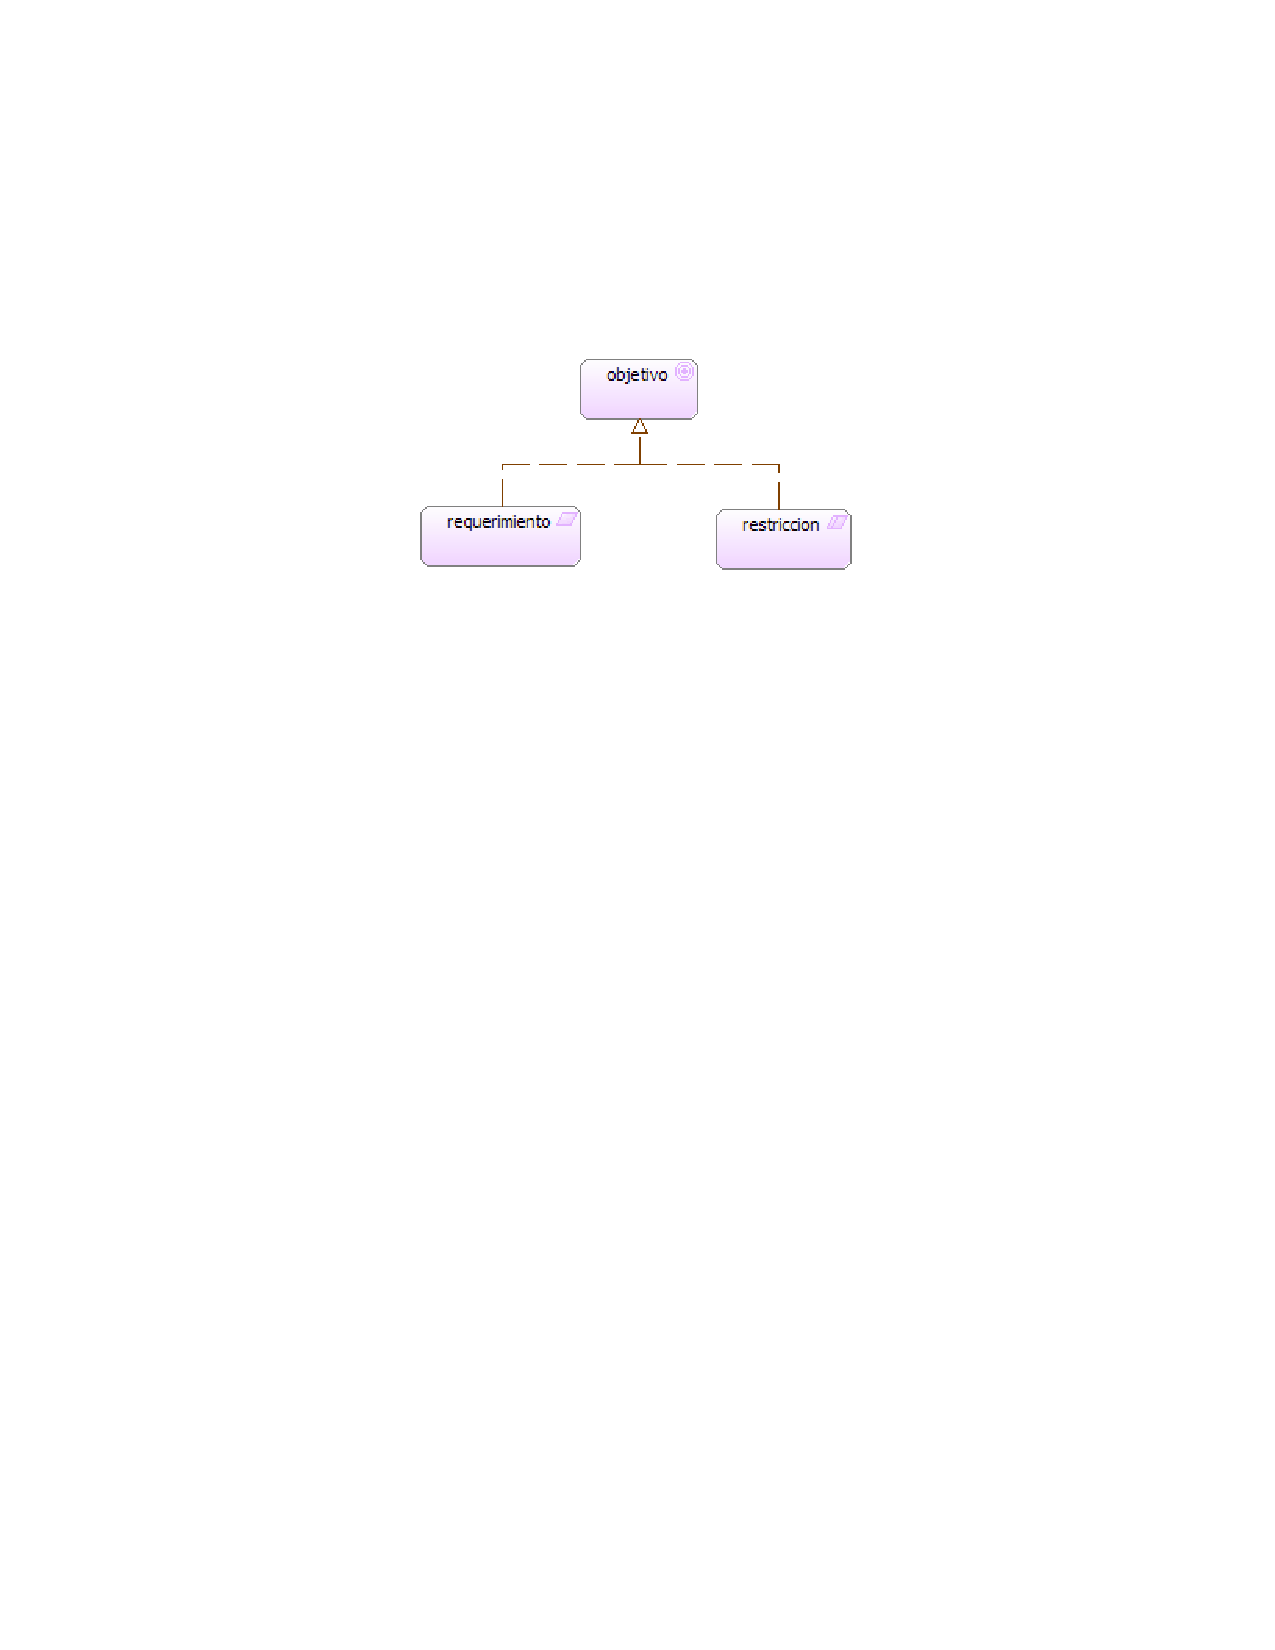
\includegraphics{realizacion_de_requerimientos}
\caption{Metamodelo del punto de vista de realización de requisitos.}
\end{figure}

Los requisitos que realizan a los objetivos más importantes se materializan en tres: Valorar una marca, comparar diferentes marcas y gestionar la información de una marca.

\begin{figure}[h]
\centering
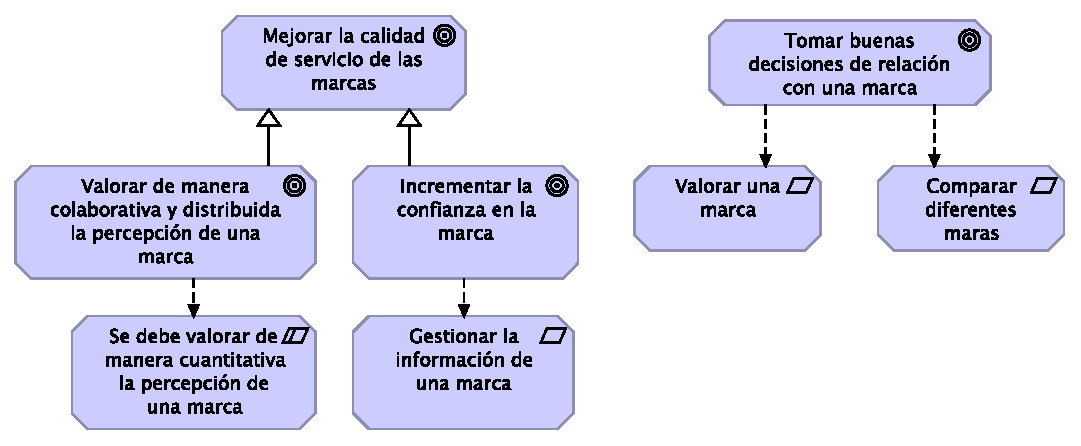
\includegraphics[scale=0.70]{MRealizacionrequerimientos}
\caption{Punto de vista de realización de requisitos.}
\end{figure}


\section{Motivación}
La motivación punto de vista permite al diseñador o analista modelar el aspecto de la motivación, sin centrarse en determinados elementos dentro de este aspecto. Por ejemplo, este punto de vista se puede utilizar para presentar una visión completa o parcial del aspecto motivación en la relación de las partes interesadas, sus objetivos principales, los principios que aplican, y los principales requerimientos de servicios, procesos, aplicaciones y objetos.

\begin{figure}[H]
\centering
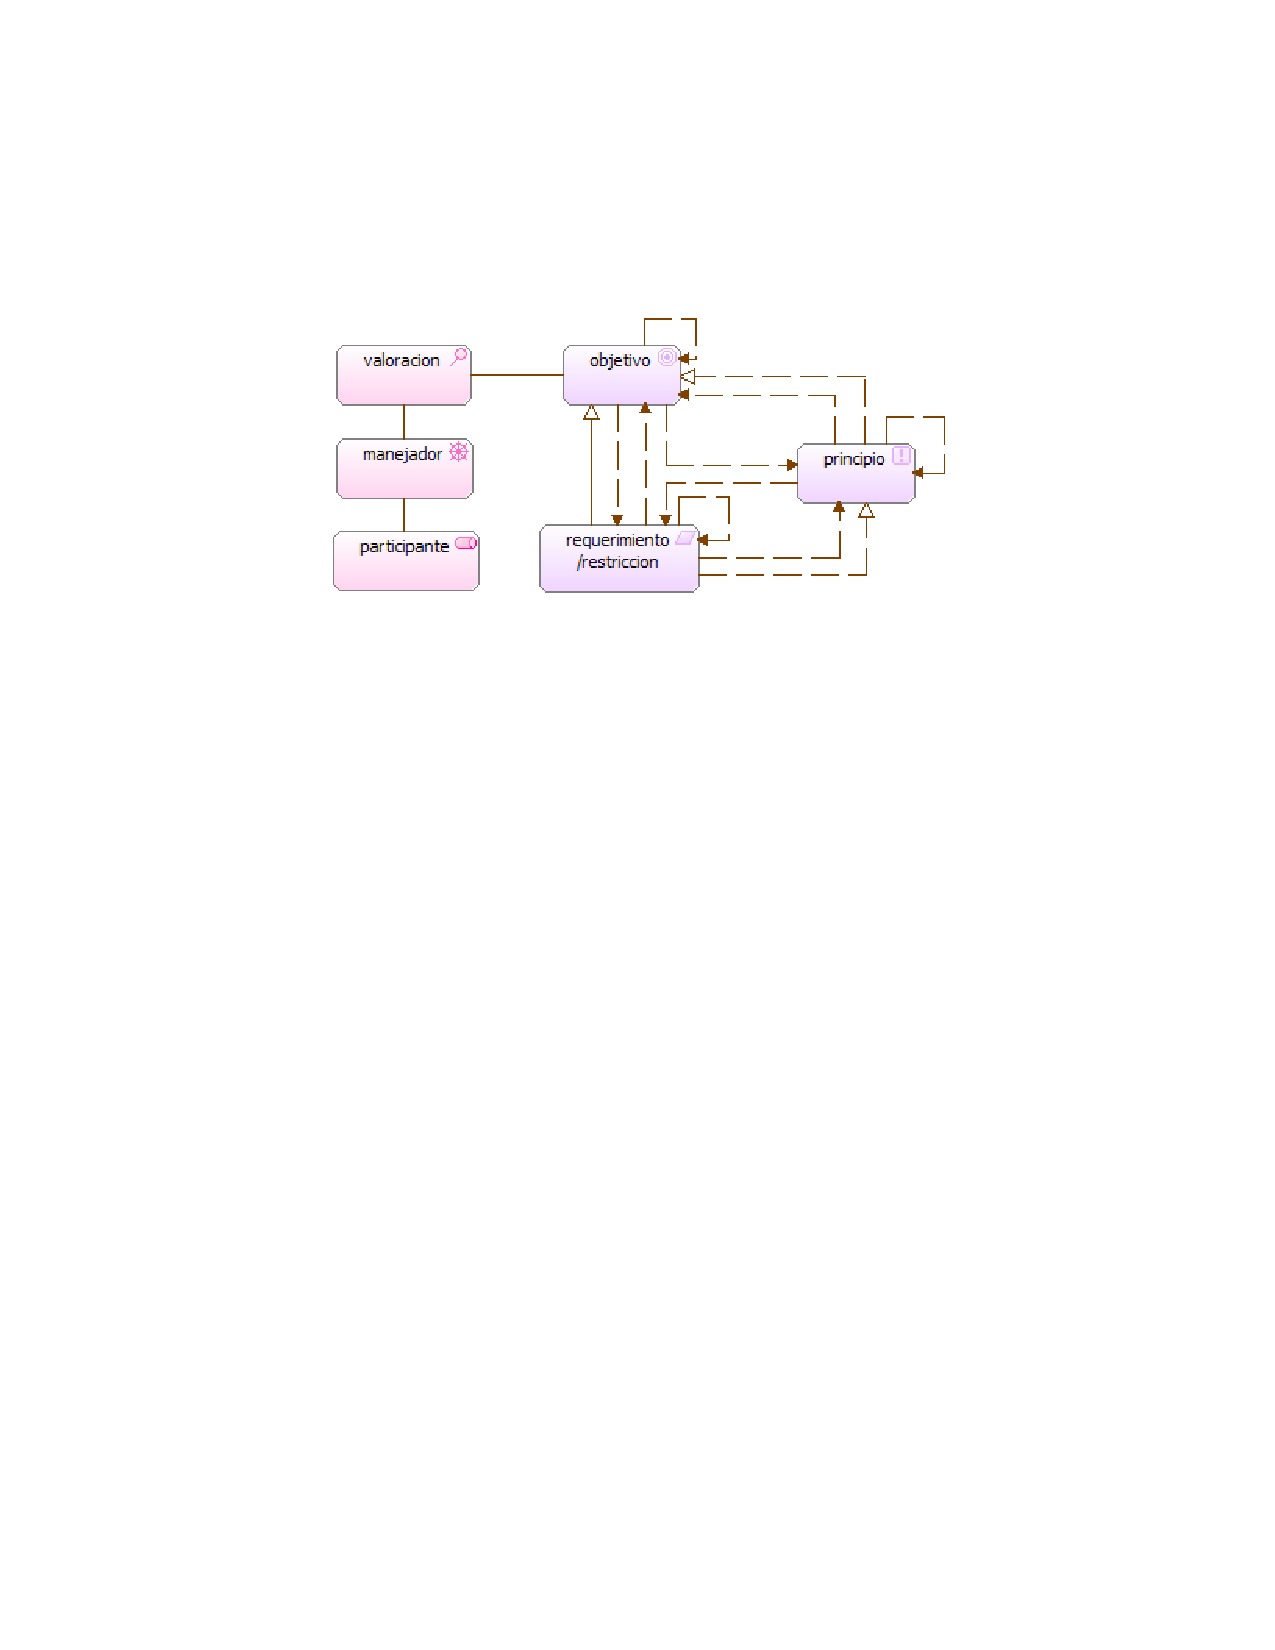
\includegraphics{motivacion}
\caption{Metamodelo del punto de vista de motivación.}
\end{figure}

Se puede observar en la figura del punto de vista de motivación \ref{mmotivacion}, que los manejadores más importantes que deben ser tenidos en cuenta en este negocio son: mejora continua de la marca y satisfacción del usuario. 

\begin{figure}[H]
\centering
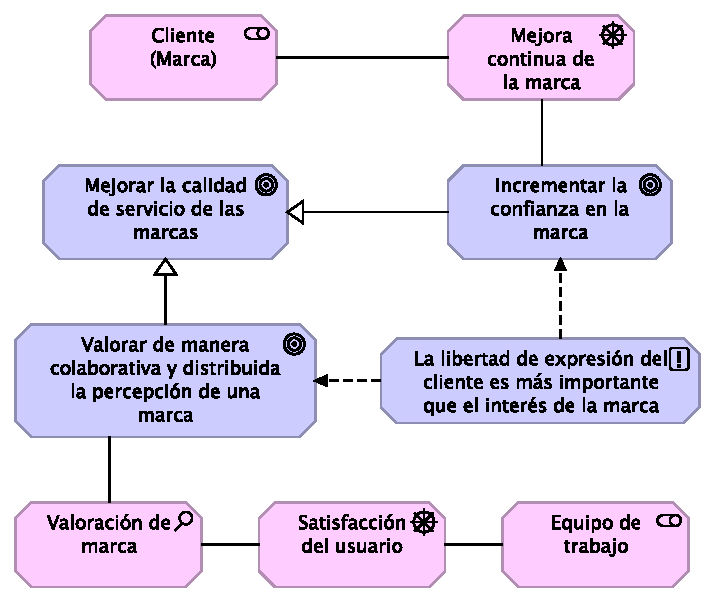
\includegraphics[scale=0.8]{MMotivacion}
\caption{Punto de vista de motivación.}
\label{mmotivacion}
\end{figure}


\section{Proyecto}
Un punto de vista del proyecto se utiliza principalmente para modelar la gestión del cambio de arquitectura. La \textit{arquitectura} del proceso de migración de una vieja situación (estado actual de arquitectura empresarial) a una nueva situación deseada (objetivo de arquitectura de la empresa) tiene consecuencias importantes sobre el subsiguiente proceso de toma de decisiones de la estrategia de crecimiento a largo plazo y medio. 

\begin{figure}[H]
\centering
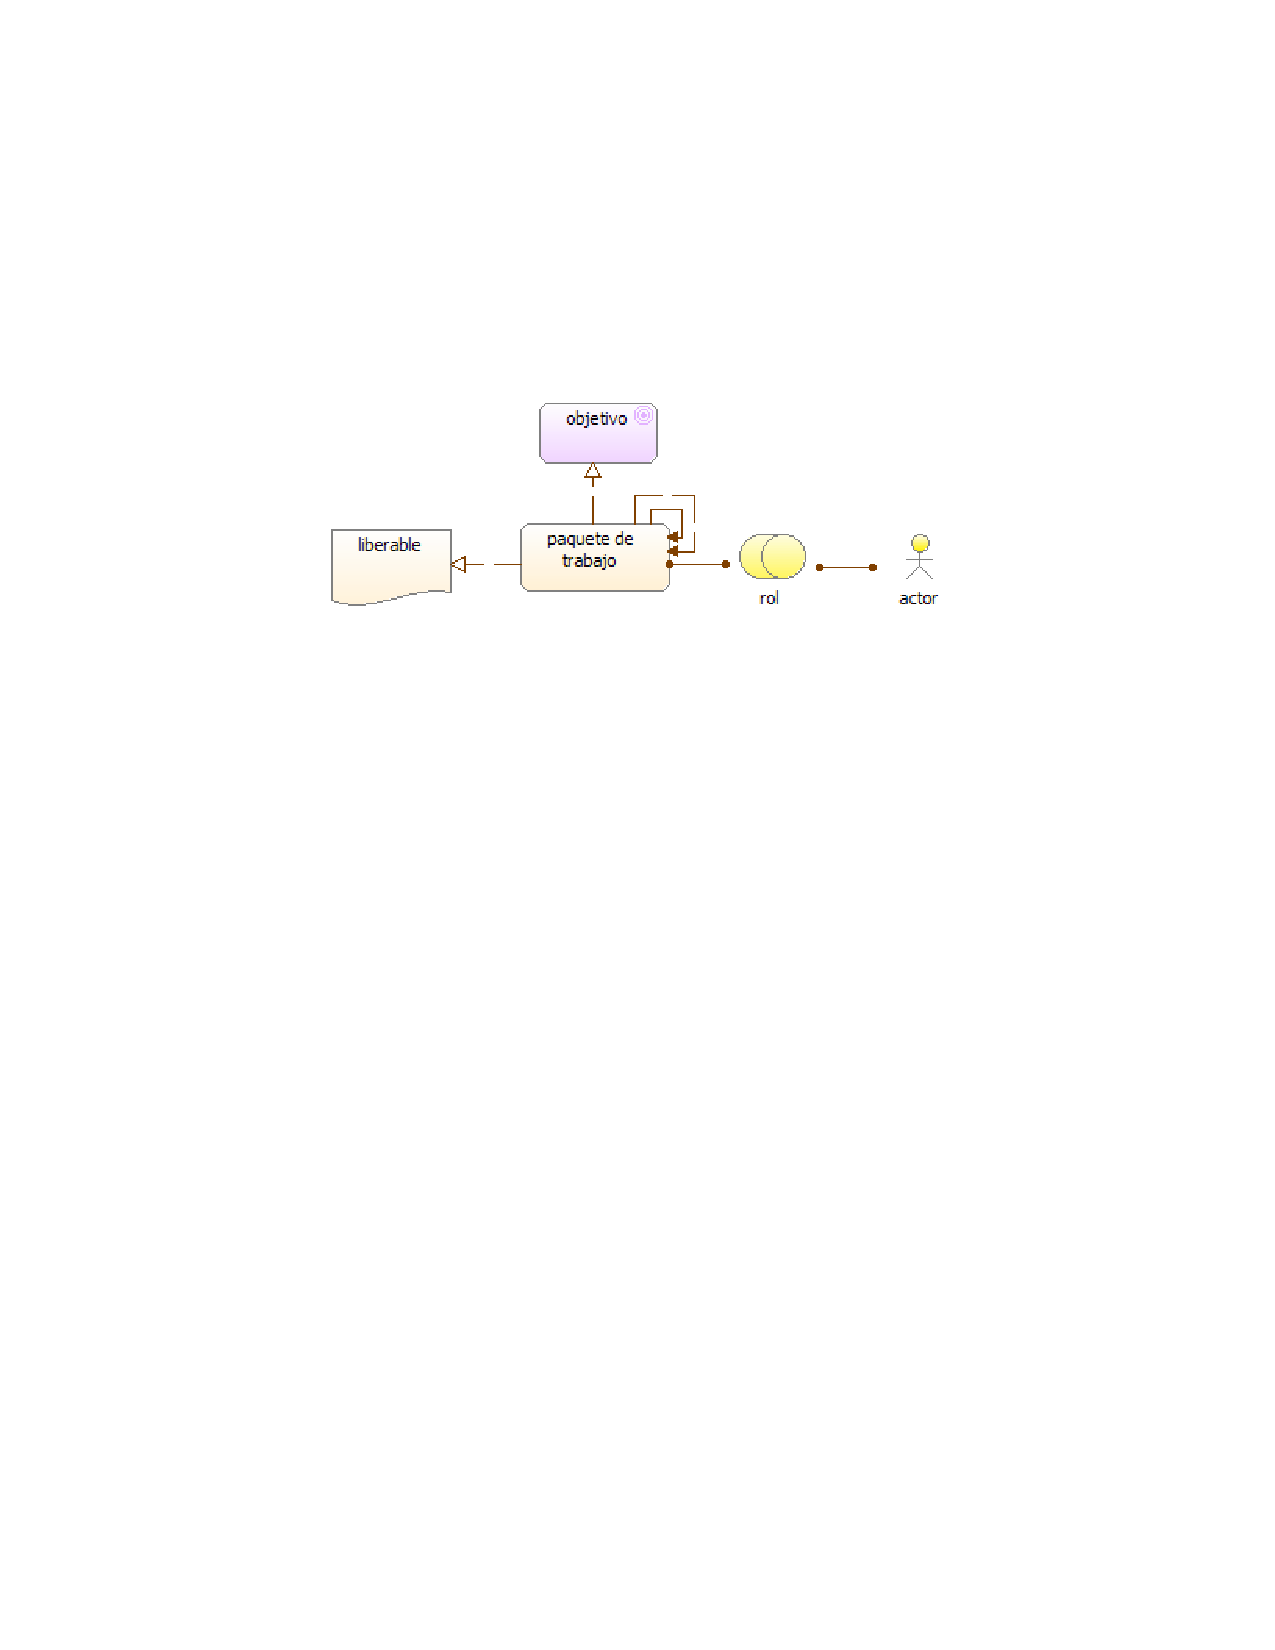
\includegraphics{proyecto}
\caption{Metamodelo del punto de vista de proyecto.}
\end{figure}

Algunas de las decisiones que deben ser tomadas en cuenta por los modelos diseñados en este punto de vista son: 
\begin{itemize}
      \item El desarrollo de la arquitectura empresarial en toda la organización es una tarea que puede requerir varios años. 
        \item Todos los sistemas y servicios deben permanecer en funcionamiento sin tener en cuenta todas las modificaciones y presumibles cambios en la arquitectura de la empresa durante el proceso de cambio. 
        \item El proceso de cambio puede tener que lidiar con los estándares de tecnología inmadura (por ejemplo, mensajería, seguridad, datos, etc.). 
        \item El cambio tiene graves consecuencias para el personal, la cultura, la forma de trabajar y la organización.    
\end{itemize}

Además, hay varios otros aspectos de gobierno, que obstaculizaron el proceso de transformación, tales como la cooperación interna y externa, la gestión de la cartera de proyectos, gestión de proyectos (entregables, objetivos, etc.), la planificación de la platea, los aspectos financieros y legales, etc.

\marginpar{
    \begin{figure}[H]
        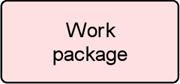
\includegraphics[scale=0.8]{Iwork_package}
    \end{figure} 
    \footnotesize 
    \textbf{Paquete de trabajo}. Una serie de acciones destinadas a lograr un objetivo único dentro de un tiempo especifico.
\newline
}
\marginpar{
    \begin{figure}[H]
        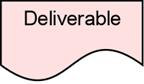
\includegraphics[scale=0.8]{Ideliverable}
    \end{figure} 
    \footnotesize 
    \textbf{Liberable}. Un resultado definido precisamente  de un paquete de trabajo.
}

Este proyecto debe ser inicialmente orientado a la construcción de la aplicación móvil de valoración de marcas con el objetivo de lograr, a partir de la valoración de los usuarios, recoger la información que permita valorar de manera colaborativa y distribuida la percepción de una marca. 

\begin{figure}[H]
\centering
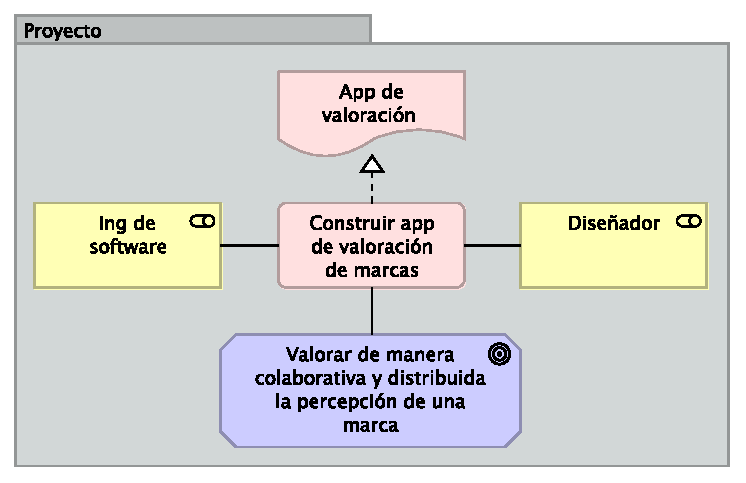
\includegraphics{MProyecto}
\caption{Punto de vista de proyecto.}
\end{figure}

\section{Migración}

El punto de vista de migración implica modelos y conceptos que se pueden utilizar para especificar la transición de una arquitectura existente a una arquitectura deseada.

\begin{figure}[H]
\centering
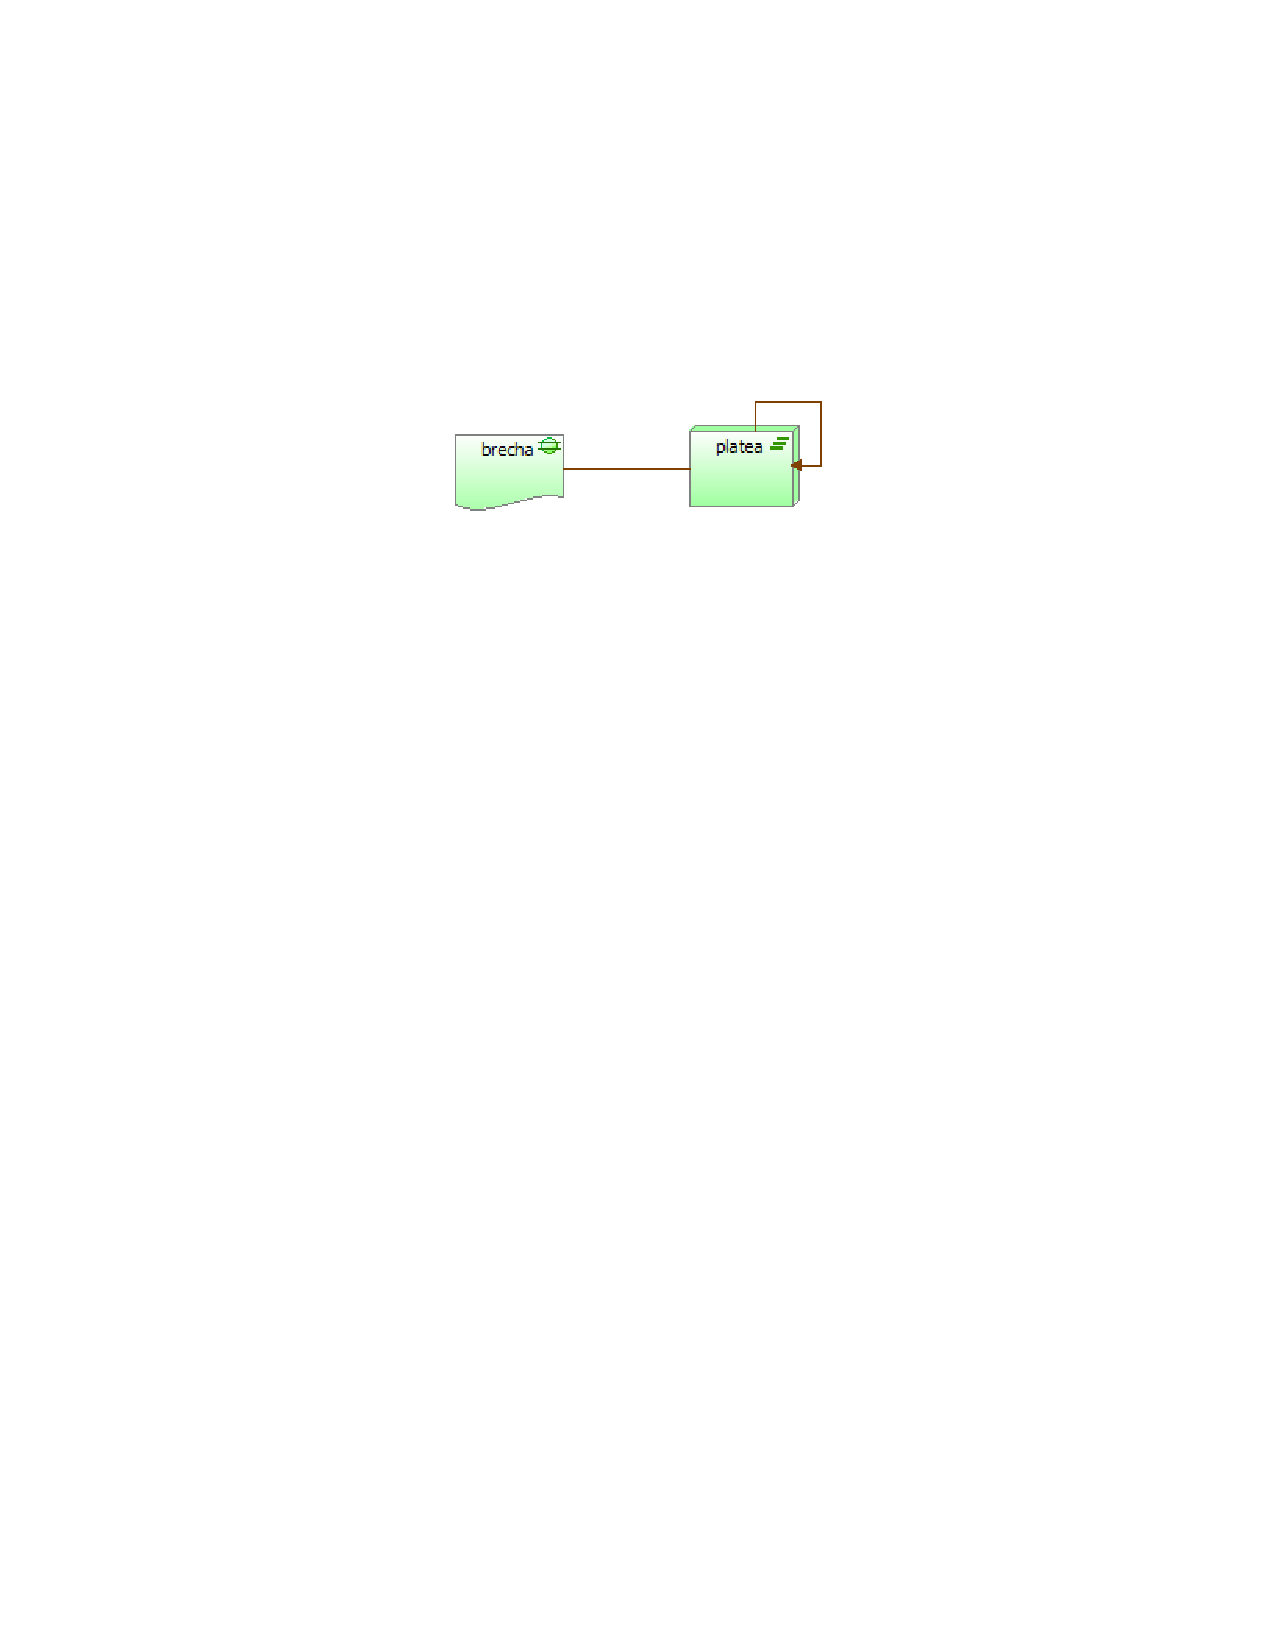
\includegraphics{migracion}
\caption{Metamodelo del punto de vista de migración.}
\end{figure}

\marginpar{
    \begin{figure}[H]
        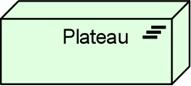
\includegraphics[scale=0.8]{Iplateau}
    \end{figure} 
    \footnotesize 
    \textbf{Platea}. Un estado relativamente estable de la arquitectura que existe durante un período de tiempo limitado.
\newline
}
\marginpar{
    \begin{figure}[H]
        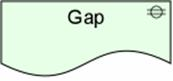
\includegraphics[scale=0.8]{Igap}
    \end{figure} 
    \footnotesize 
    \textbf{Brecha}. Uno de los resultados del análisis de la brecha entre dos plateas. 
}El producto planeado será el sistema software de valoración de marcas, pero adicionalmente se espera escalar en dos grandes plateas. Primero la personalización de ciertas valoraciones y segundo, la comunicación directa entre marcas y usuarios.

\begin{figure}[H]
\centering
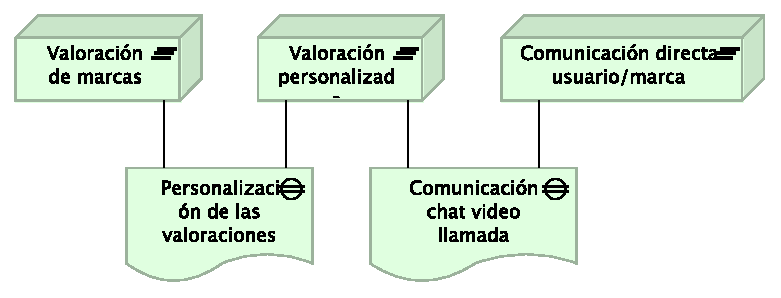
\includegraphics{MMigracion}
\caption{Punto de vista de migración.}
\end{figure}


\section{Migración e implementación}

El punto de vista de la migración y la implementación se utiliza para relacionar los programas y proyectos de las partes de la arquitectura que se implementan. Esta vista permite el modelado del alcance de los programas, proyectos, actividades del proyecto en términos de las plateas que se realizan o los elementos de la arquitectura individuales que se ven afectados. Además, la forma en que se ven afectados los elementos puede ser indicado por la anotación de las relaciones. 

\begin{figure}[H]
\centering
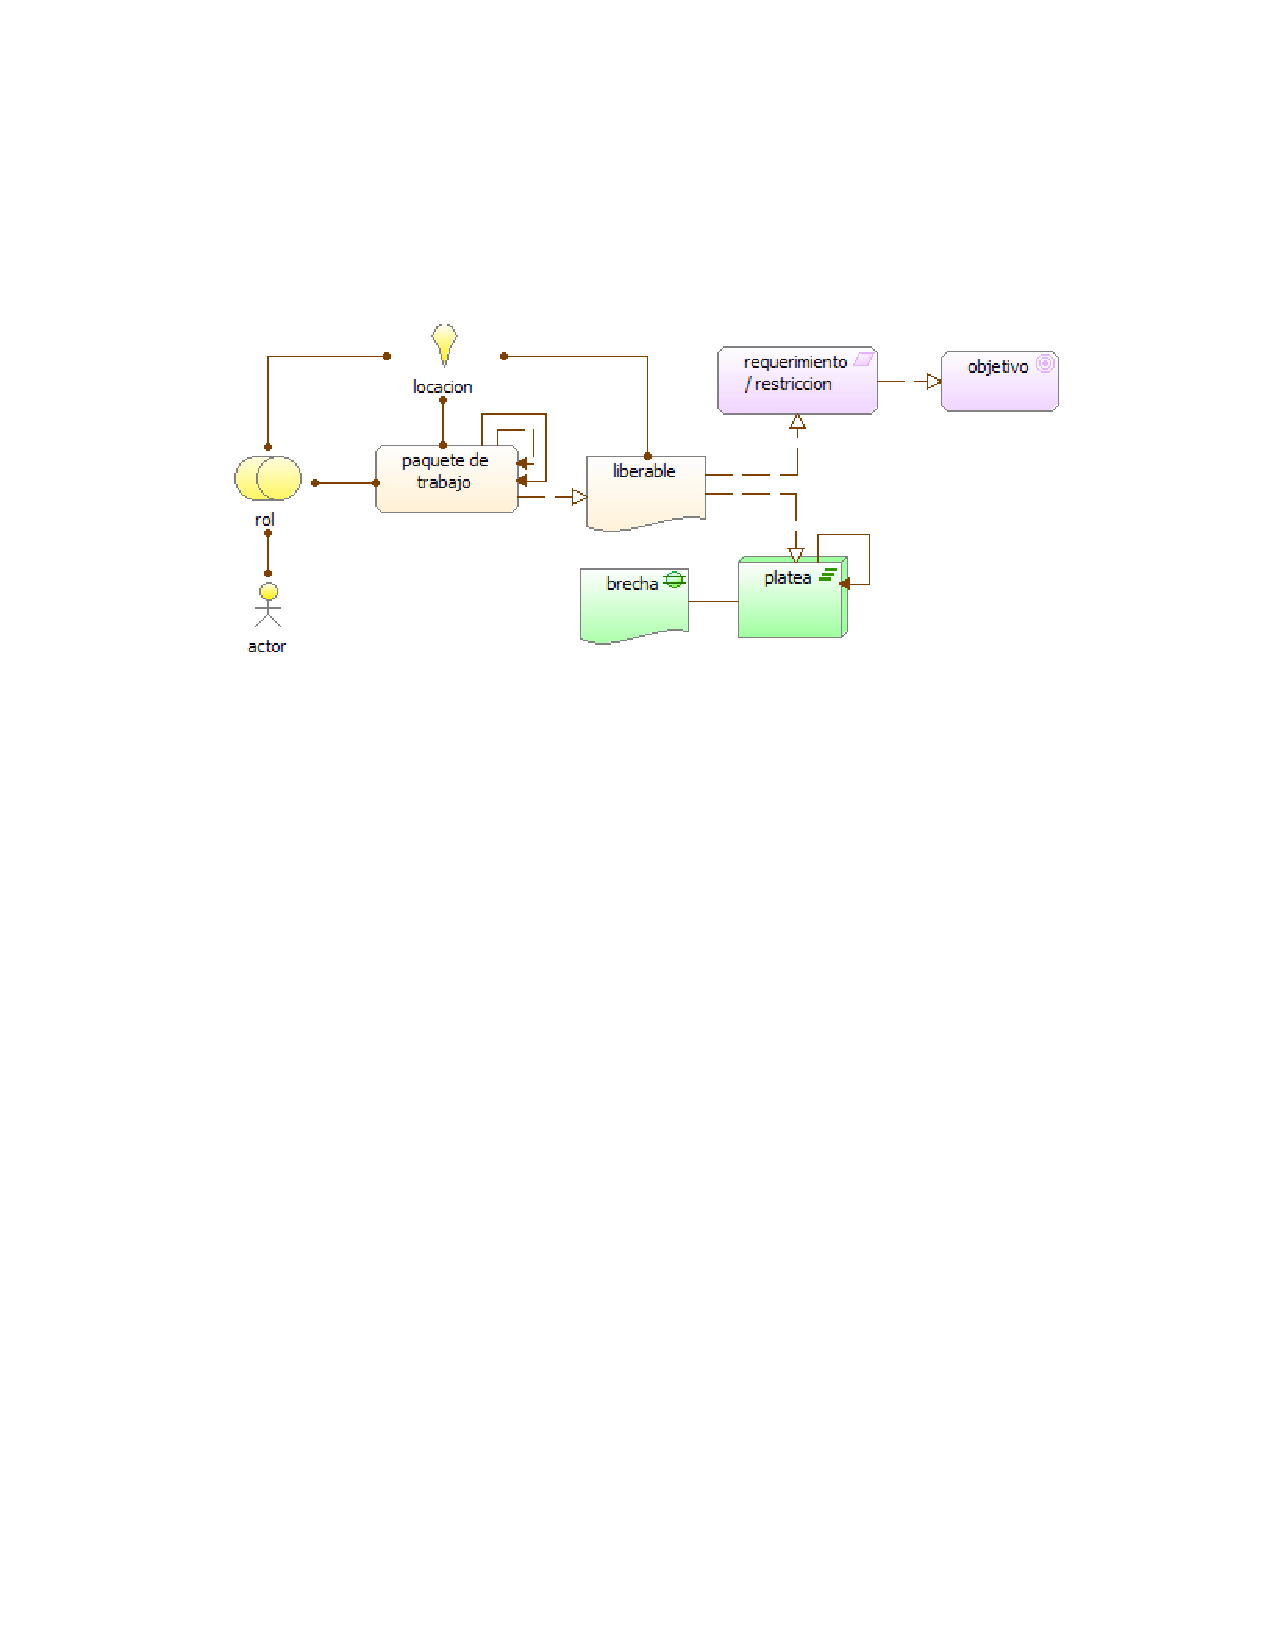
\includegraphics[scale=0.7]{migracion_e_implementacion}
\caption{Metamodelo del punto de vista de migración e implementación.}
\end{figure}

Por otra parte, este punto de vista se puede utilizar en combinación con el punto de vista de los programas y proyectos para apoyar la gestión del portafolio: 
\begin{itemize}
        \item El punto de vista de los programas y proyectos es adecuado para relacionar los objetivos de negocio a los programas y proyectos. Por ejemplo, esto hace posible el análisis a un nivel alto si todos los objetivos de negocio se cubren de manera suficiente por la portafolio actual. 
        \item El punto de vista de la implementación y la migración es adecuado para relacionar los objetivos de negocio (y requisitos) a través de programas y proyectos de (partes de) la arquitectura. Por ejemplo, esto hace posible el análisis de la posible superposición entre las actividades del proyecto o para analizar la coherencia entre las dependencias y las dependencias del proyecto entre las plateas o elementos de la arquitectura.
\end{itemize}

Como realización del objetivo principal con su restricción se debe crear un entregable principal que se materializará como la primera platea.

\begin{figure}[H]
\centering
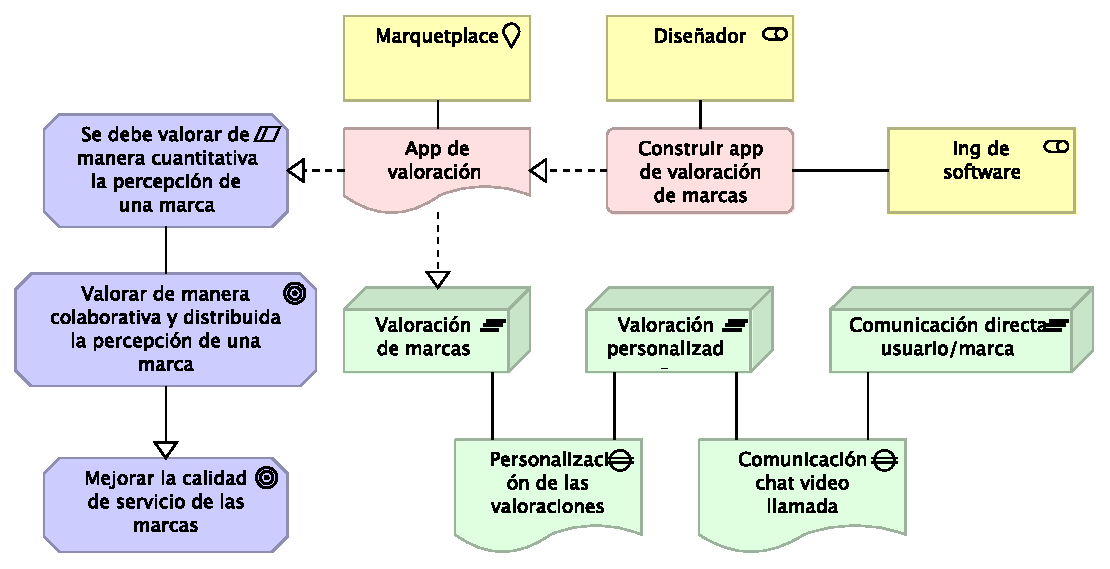
\includegraphics[scale=0.7]{MMigracioneimplementacion}
\caption{Punto de vista de migración e implementación.}
\end{figure}


%*******************************************************
% Capitulo seis
%*******************************************************

\chapter{Capa de negocio}

\marginpar{
    \begin{figure}[H]
        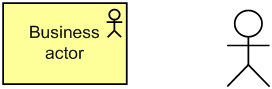
\includegraphics[scale=0.6]{IBusiness_actor}
    \end{figure} 
    \footnotesize 
    \textbf{Actor}. Una entidad organizacional que es capaz de ejecutar un comportamiento.
\newline
}
\marginpar{
    \begin{figure}[H]
        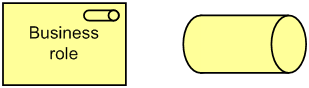
\includegraphics[scale=0.6]{IBusiness_role}
    \end{figure} 
    \footnotesize 
    \textbf{Rol}. La responsabilidad de llevar a cabo un comportamiento específico, al que se le puede asignar un actor.
\newline    
}
\marginpar{
    \begin{figure}[H]
        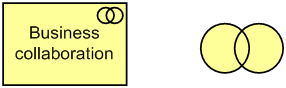
\includegraphics[scale=0.6]{IBusiness_collaboration}
    \end{figure} 
    \footnotesize 
    \textbf{Colaboración}.Un agregado de dos o más funciones de negocios que trabajan en conjunto para llevar a cabo un comportamiento colectivo.
}

\section{Organización}

El punto de vista de organización se centra en la organización de una empresa, un departamento, una red de empresas o cualquier otra entidad organizativa. Es posible presentar los modelos de este punto de vista como diagramas de bloques anidados o de una manera mas tradicional a través de un organigrama. Este punto de vista es muy útil en la identificación de las competencias, la autoridad y las responsabilidades dentro de la organización. 


\begin{figure}[h]
\centering
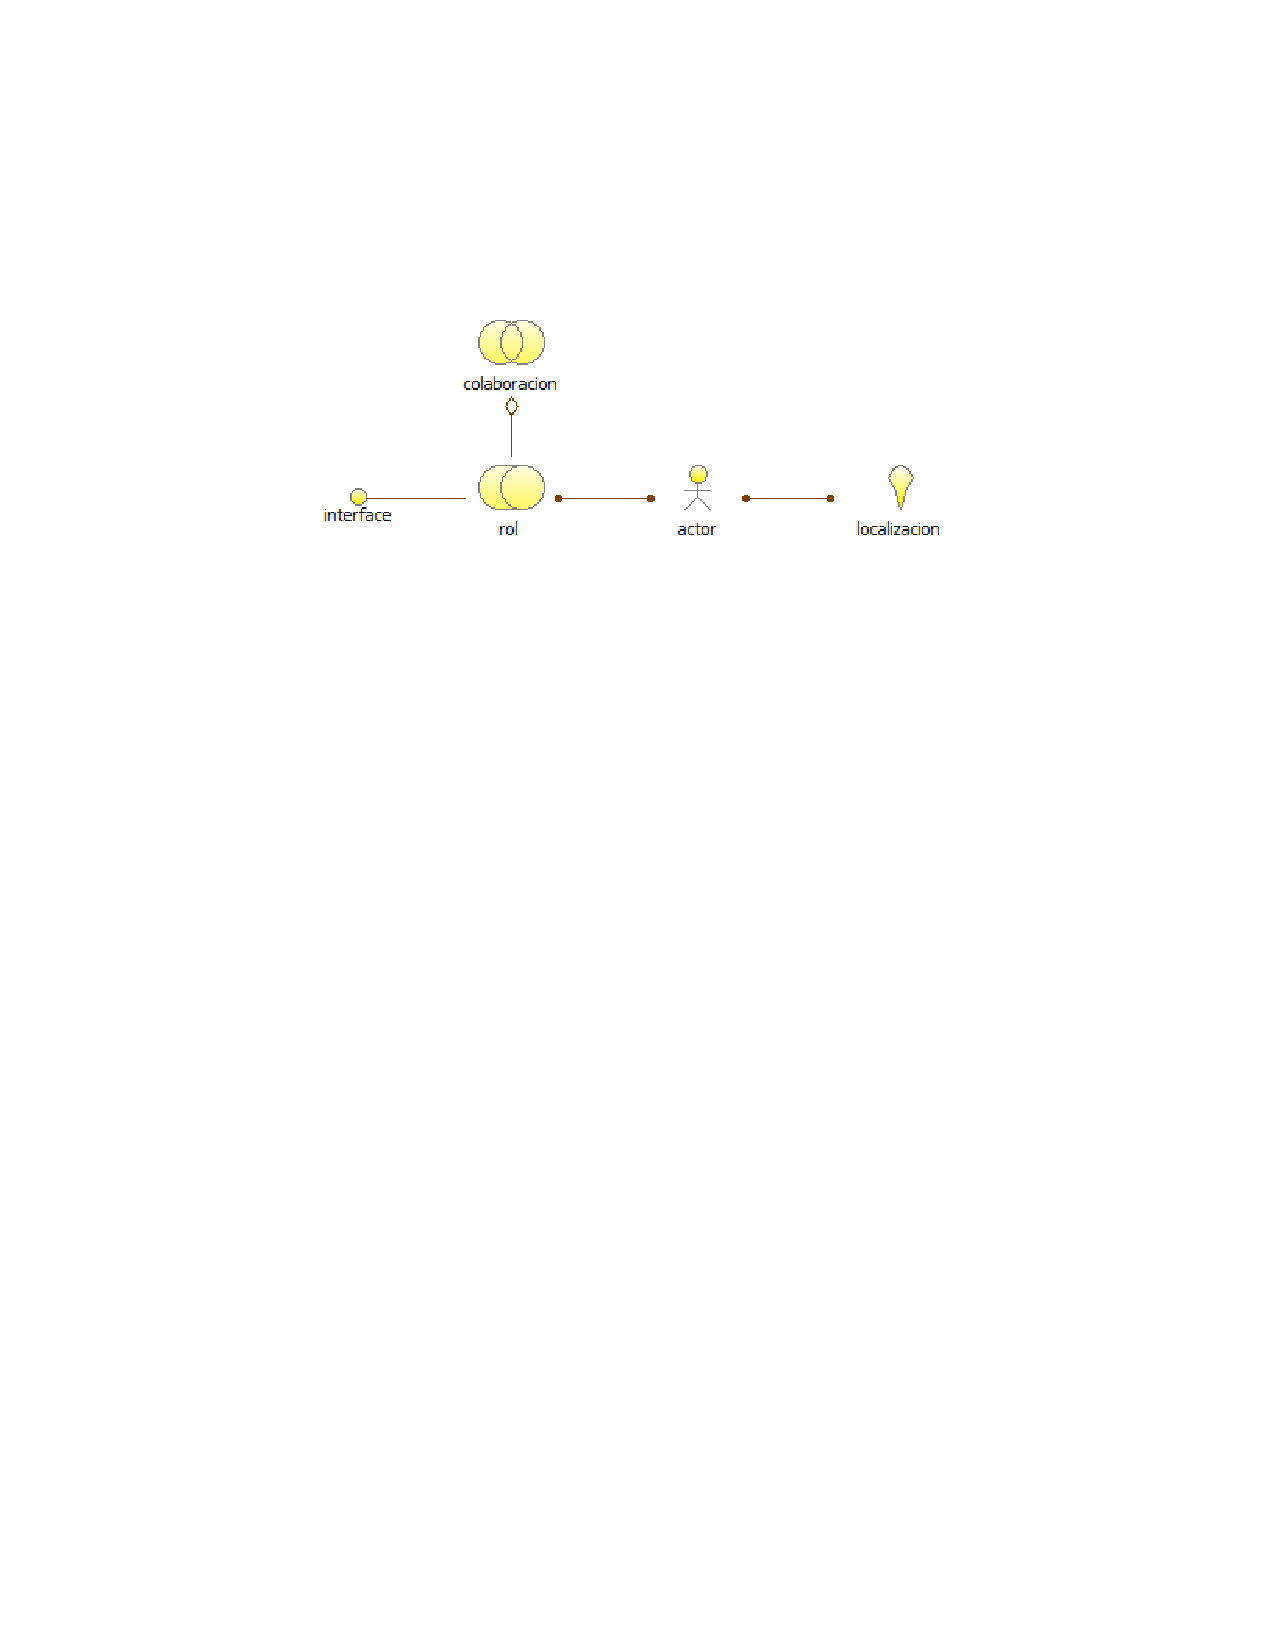
\includegraphics{organizacion}
\caption{Metamodelo del punto de vista organización.}
\end{figure}

En función del cumplimiento de los objetivos planteados, se propone la siguiente estructura organizacional para desarrollar el negocio.

\begin{figure}[h]
\centering
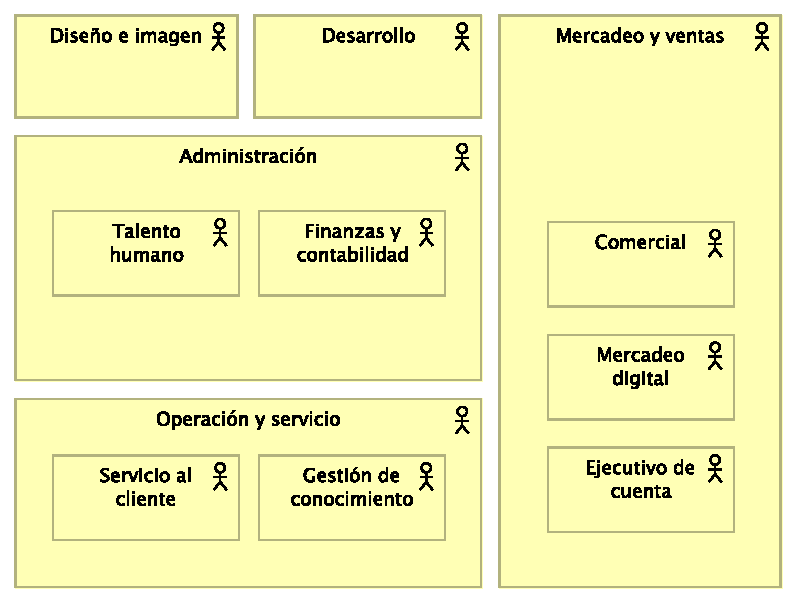
\includegraphics{Morganizacion}
\caption{Punto de vista organización.}
\end{figure}
 
\section{Cooperación de actor}

\marginpar{
    \begin{figure}[H]
        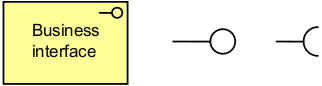
\includegraphics[scale=0.6]{ibusiness_interfaz}
    \end{figure} 
    \footnotesize 
    \textbf{Interfaz}.Un punto de acceso donde se pone a disposición un servicio de negocio para el entorno.
\newline
}
\marginpar{
    \begin{figure}[H]
        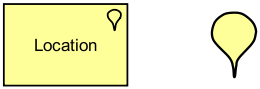
\includegraphics[scale=0.6]{ilocacion}
    \end{figure} 
    \footnotesize 
    \textbf{Ubicación}. Un lugar conceptual en el espacio.
\newline    
}


El punto de vista de cooperación de actor se centra en las relaciones de los actores entre sí y con su entorno. Un ejemplo común de esto es el "diagrama de contexto", lo que pone una organización con su entorno, que consiste en las partes externas, tales como clientes, proveedores y otros socios comerciales.Es muy útil en la determinación de dependencias externas y colaboraciones y muestra la cadena de valor o de la red en el que opera el actor. 

Otro uso importante es mostrar cómo una serie de actores comerciales y/o componentes de la aplicación en conjunto cooperan para realizar un proceso de negocio. Por lo tanto, en este punto de vista,le puede aplicar tanto a los actores comerciales o funciones y a los componentes de la aplicación.

\begin{figure}[h]
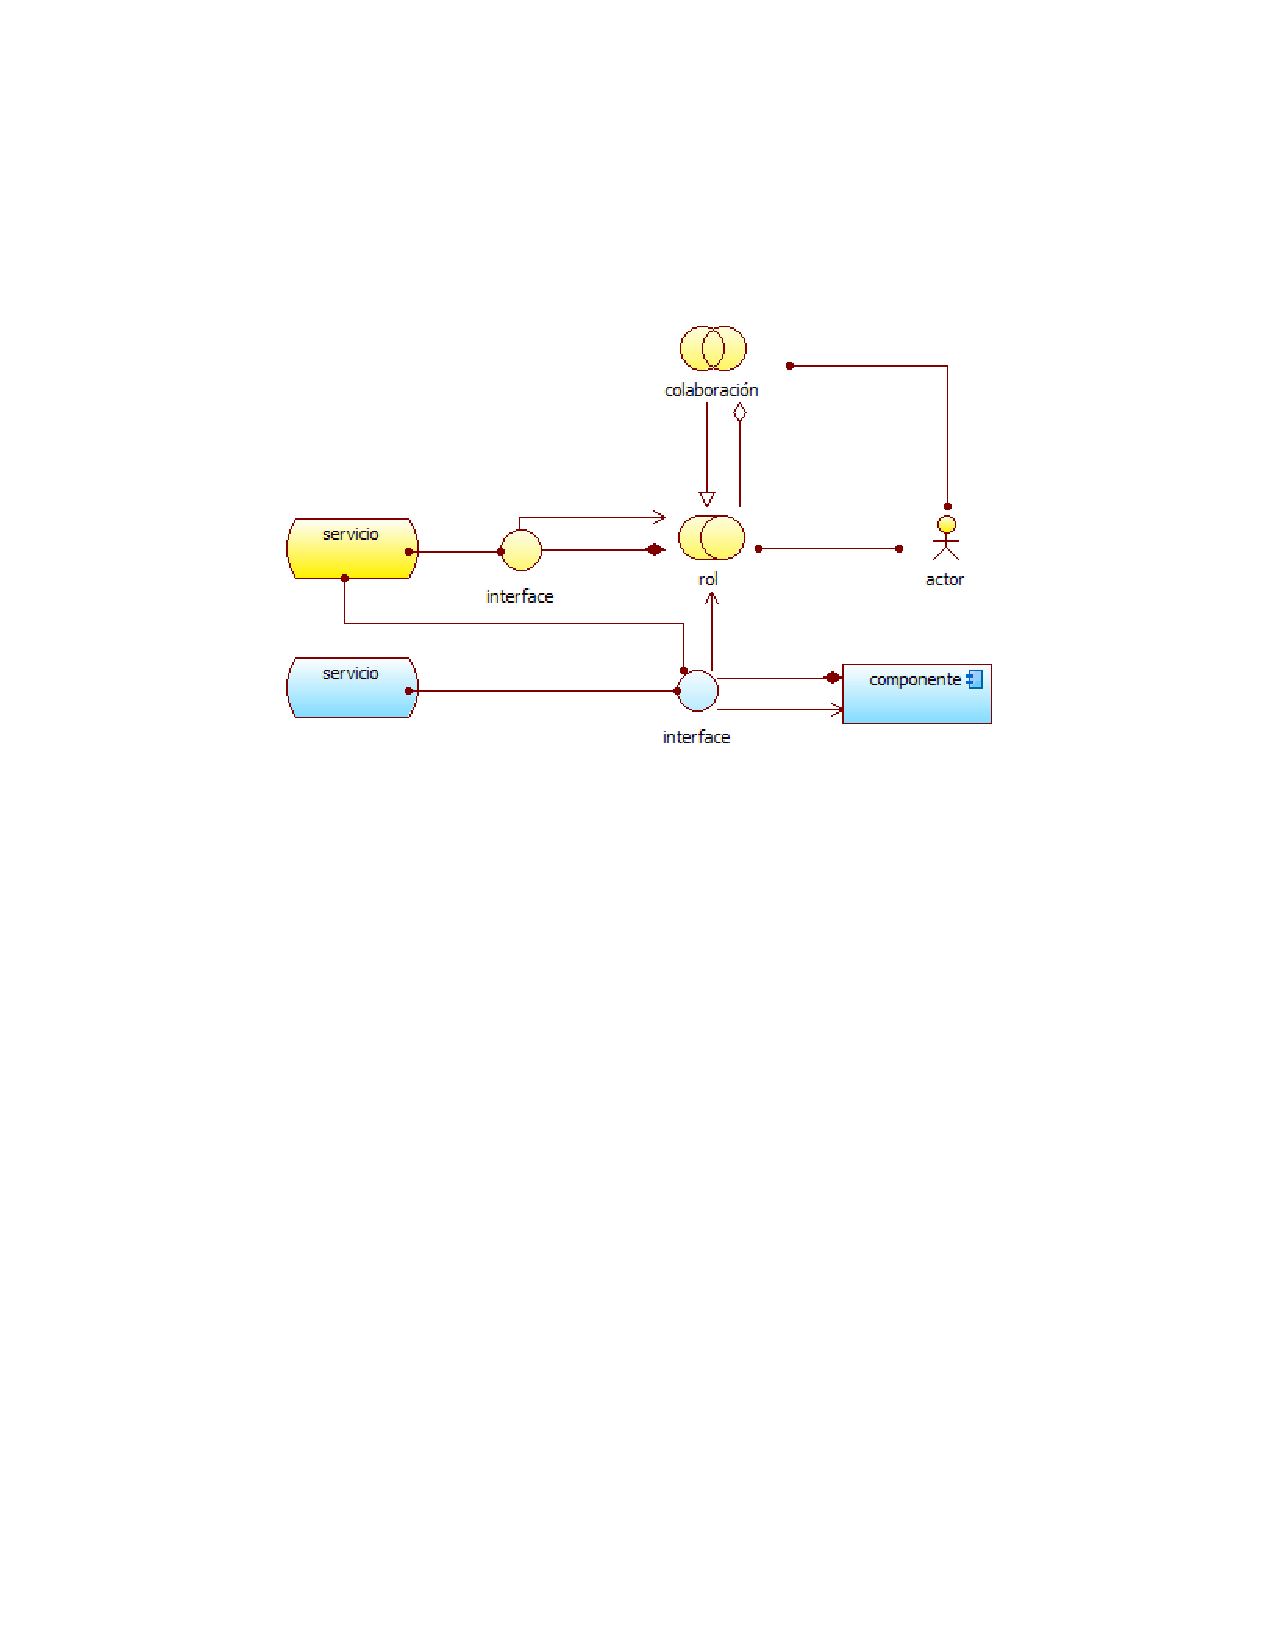
\includegraphics[scale=0.7]{cooperacion}
\centering
\caption{Metamodelo del punto de vista de cooperación de Actor.}
\end{figure}

Los stakeholders clave mantienen una relación con la estructura organizacional que se puede observar en la figura \ref{mcooperacionactor}.

\begin{figure}[h] 
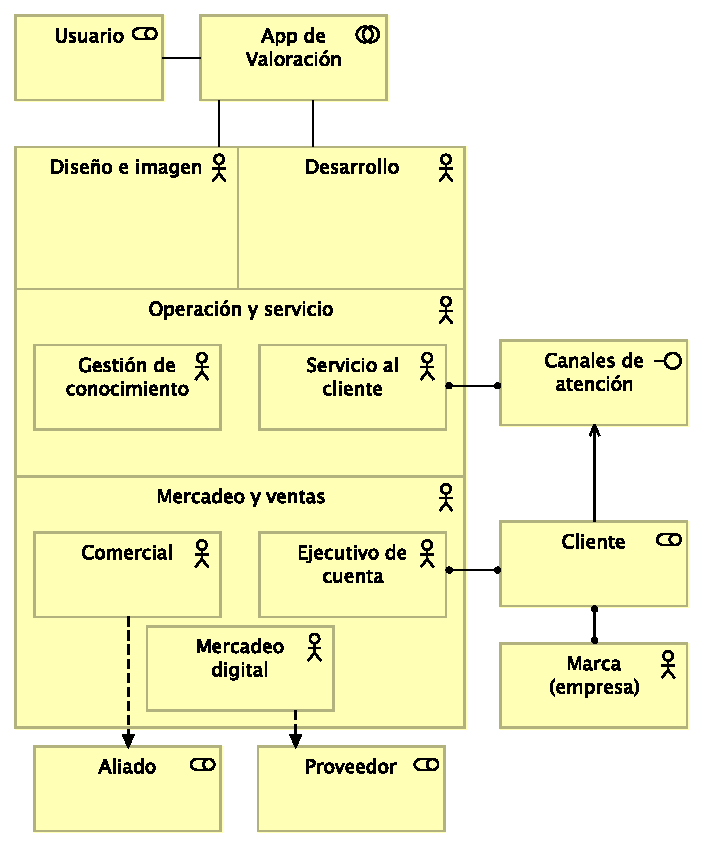
\includegraphics[scale=0.7]{Mcooperacionactor}
\centering
\caption{Punto de vista de cooperación de Actor.}
\label{mcooperacionactor}
\end{figure}

\section{Función de negocio}

\marginpar{
    \begin{figure}[H]
        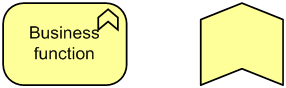
\includegraphics[scale=0.6]{ibusiness_funcion}
    \end{figure} 
    \footnotesize 
    \textbf{Función}. Un elemento de comportamiento que agrupa comportamientos basado en un conjunto seleccionado de criterios (por lo general requiere recursos de la empresa y/o competencias).
\newline
}El punto de vista de funciones de negocios muestra las principales funciones de negocio de una organización y sus relaciones en términos de los flujos de información, el valor, y bienes entre ellos. Este punto de vista es empleado para representar los aspectos más estables de una empresa en términos de las actividades primarias que realiza, independientemente de los cambios de organización o desarrollos tecnológicos. Por lo tanto, la arquitectura función de negocio de las empresas que operan en el mismo mercado a menudo presentan grandes similitudes. De esta manera, el punto de vista de la función empresarial proporciona una visión de alto nivel en las operaciones generales de la empresa, y se puede utilizar para identificar las competencias necesarias, o para estructurar una organización de acuerdo a sus actividades principales. El metamodelo se puede observar en la Figura \ref{funcion_de_negocio}.

\begin{figure}[H]   
\centering
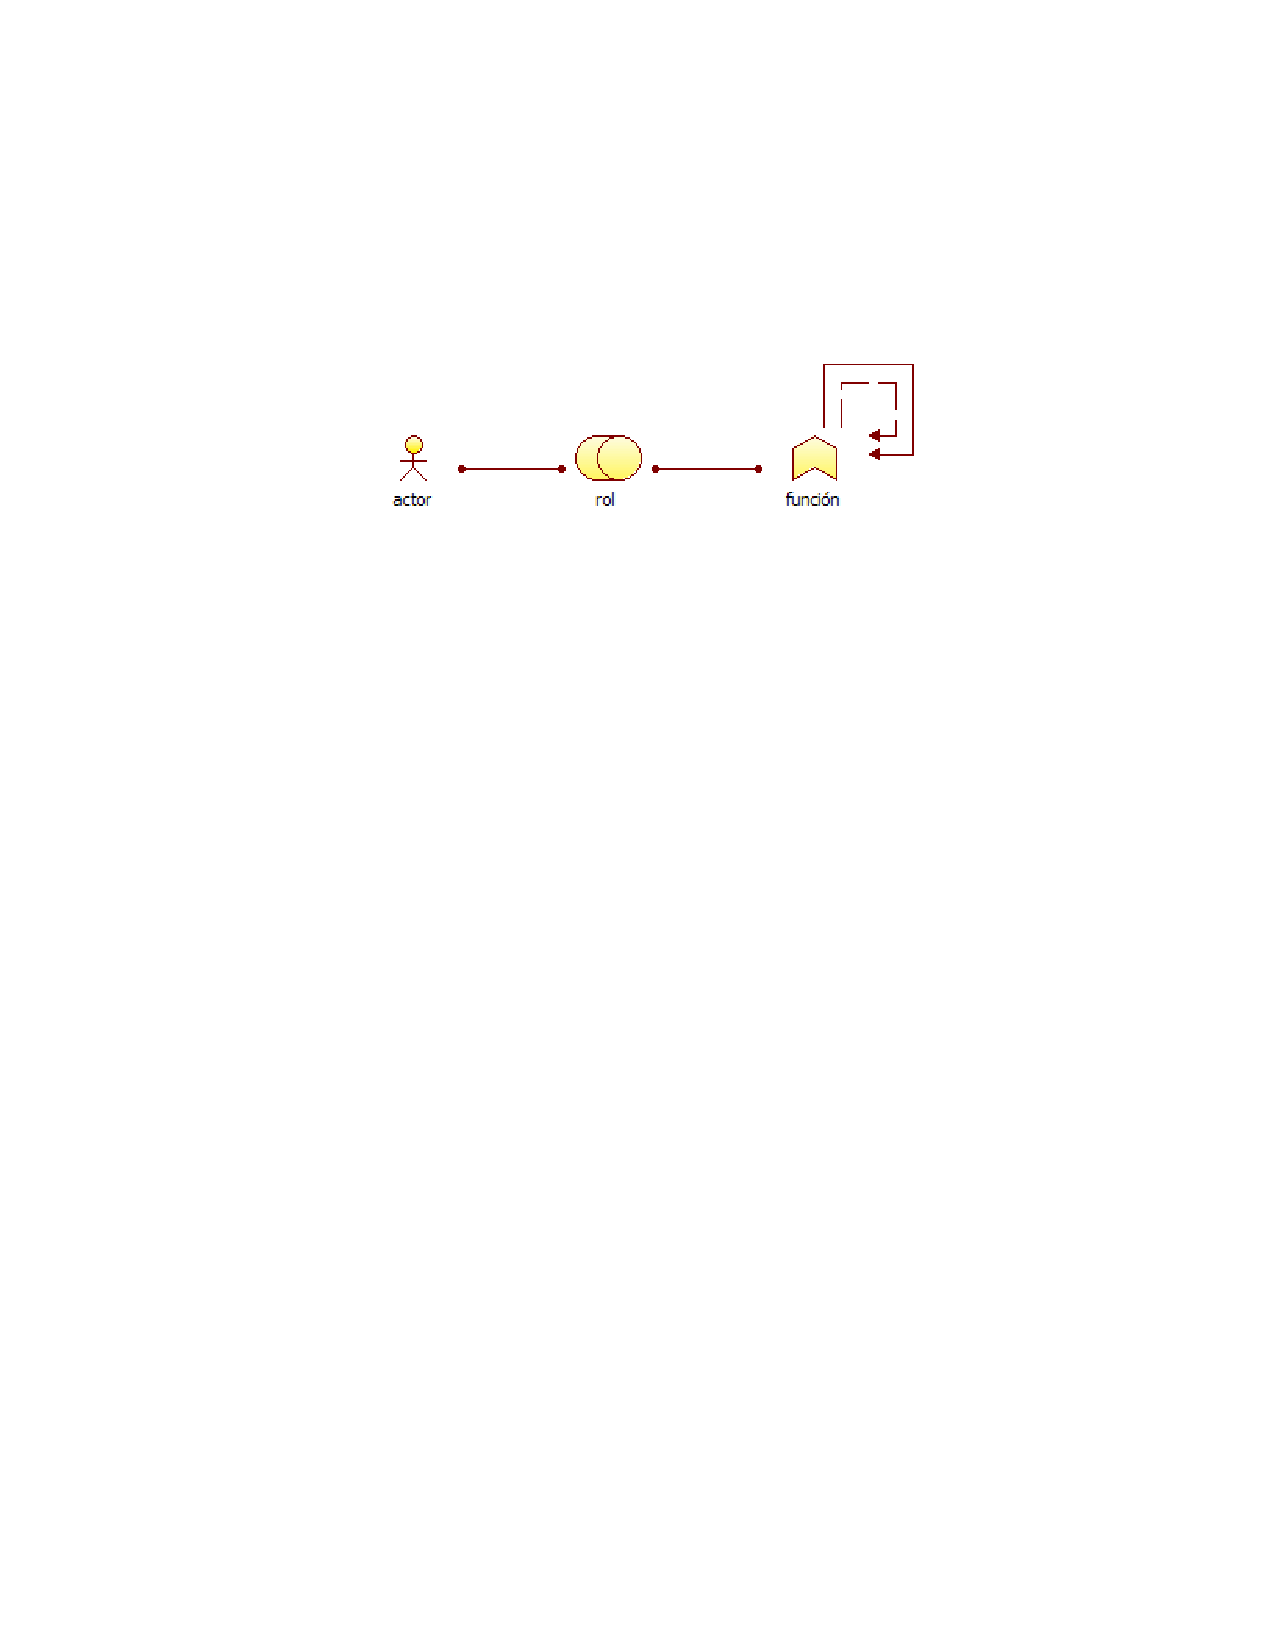
\includegraphics{funcion_de_negocio}
\caption{Metamodelo del punto de vista de función de negocio.}
\label{funcion_de_negocio}
\end{figure}

Como parte de las funciones principales con algunos interesados se tiene la compra de servicios de tecnología como ads de publicidad o servicios de cloud y mantener alto el relacionamiento con los clientes. Esta lista de posibilidades de relación se puede consultar en la descripción canvas del relacionamiento con el cliente.

\begin{figure}[H]   
\centering
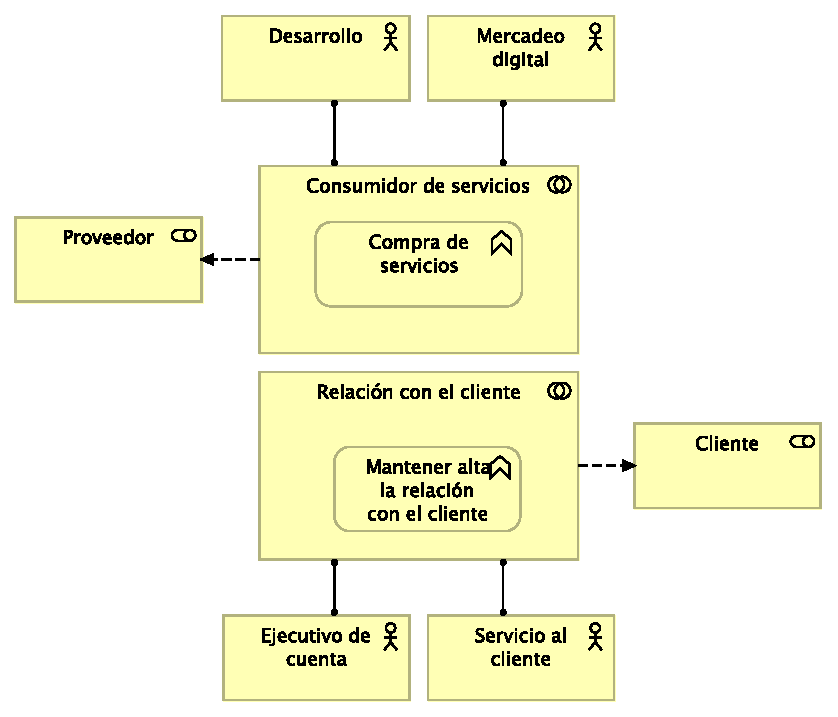
\includegraphics{MFuncionnegocio}
\caption{Punto de vista de función de negocio.}
\label{MFuncionnegocio}
\end{figure}


\section{Proceso de Negocio}


\marginpar{
    \begin{figure}[H]
        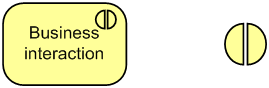
\includegraphics[scale=0.6]{ibusiness_interaccion}
    \end{figure} 
    \footnotesize 
    \textbf{Interacción}.Un elemento de comportamiento que describe el comportamiento de una colaboración.
\newline    
}
El punto de vista de procesos de negocio se utiliza para mostrar una estructura de alto nivel y la composición de uno o más procesos de negocio. Al lado de los mismos procesos, este punto de vista contiene otros conceptos directamente relacionados, como:
\marginpar{
    \begin{figure}[H]
        
\includegraphics[scale=0.6]{ibusiness_evento}
    \end{figure} 
    \footnotesize 
    \textbf{Evento}.Algo que sucede (interna o externa) e influye en el comportamiento.
    \\
}

\marginpar{
    \begin{figure}[H]
        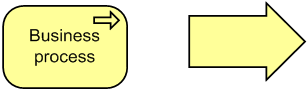
\includegraphics[scale=0.6]{ibusiness_proceso}
    \end{figure} 
    \footnotesize 
    \textbf{Proceso}. Un elemento de comportamiento que agrupa comportamientos basado en un ordenamiento de actividades.
}
\begin{itemize}
        \item Los servicios que ofrece un proceso de negocio con el mundo exterior, que muestra cómo un proceso contribuye a la realización de productos de la compañía.
        \item La asignación de los procesos de negocio a los roles, lo que da una idea de las responsabilidades de los actores asociados.
        \item La información utilizada por el proceso de negocio. 
\end{itemize}
Cada uno de ellos puede ser considerado como un "sub -view" de la vista de procesos de negocio.

\begin{figure}[H]
\centering
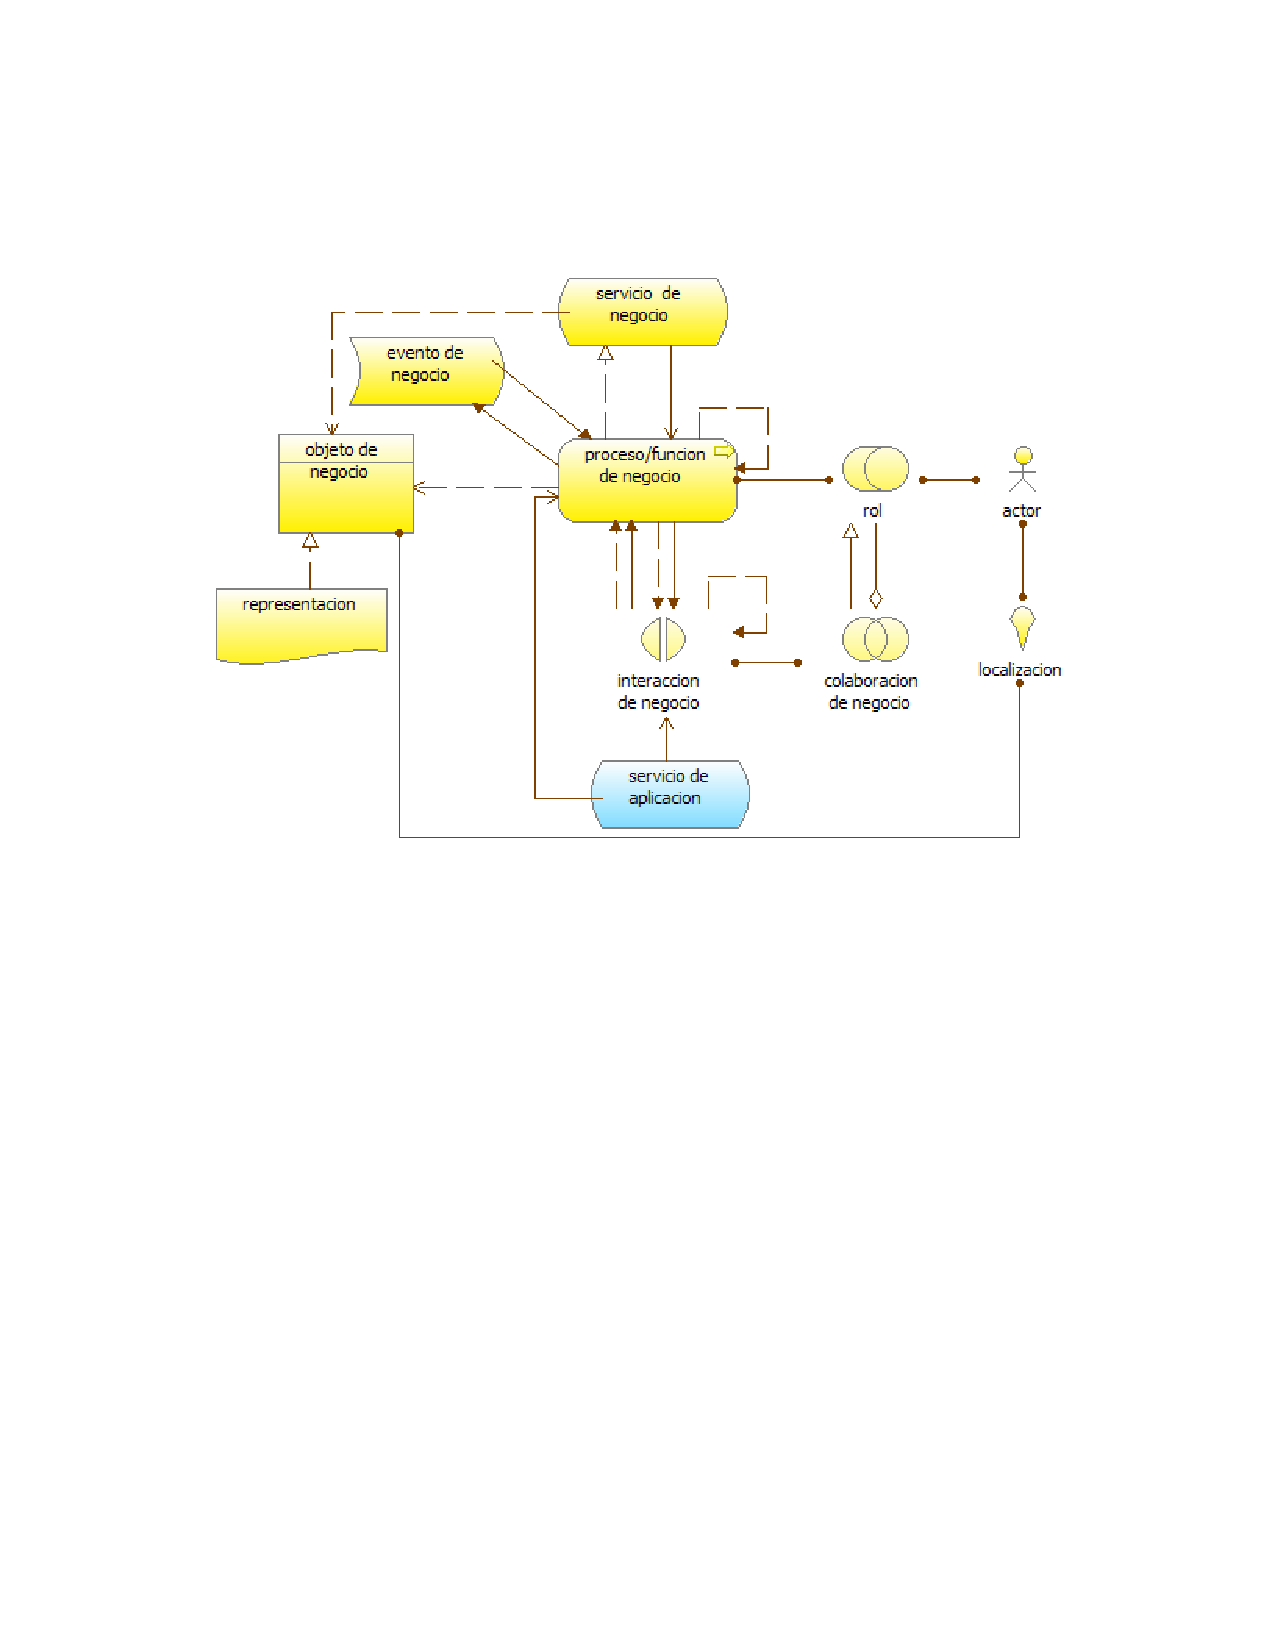
\includegraphics[scale=0.7]{proceso_de_negocio}
\caption{Punto de vista de proceso de negocio.}
\end{figure}

Se plantea entonces para esta propuesta los procesos más importantes frente al uso de la aplicación sin que sean menos relevantes la gestión comercial, el consumo de servicios de tecnología, las actividades de relacionamiento u otras descritas por el canvas. Son las actividades que hacen del uso de la aplicación un factor diferencial en proceso de negocio.

\begin{figure}[H]
\centering
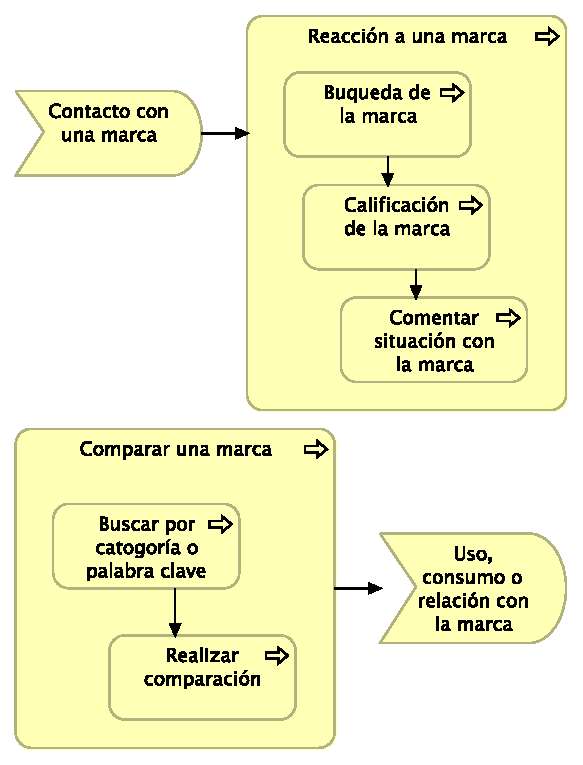
\includegraphics[scale=0.8]{MProcesonegocio}
\caption{Metamodelo del punto de vista de proceso de negocio.}
\end{figure}

\marginpar{
    \begin{figure}[H]
        
\includegraphics[scale=0.6]{ibusiness_servicio}
    \end{figure} 
    \footnotesize 
    \textbf{Servicio}.Un servicio que satisface una necesidad para un cliente (interno o externo de la organización).
\newline
}
\marginpar{
    \begin{figure}[H]
        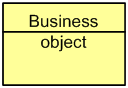
\includegraphics[scale=0.8]{ibusiness_objeto}
    \end{figure} 
    \footnotesize 
    \textbf{Objeto}.Un elemento pasivo que es relevante desde una perspectiva de negocio. 
\newline    
}


\section{Cooperación de proceso de negocio}
El punto de vista de cooperación de proceso de negocio se utiliza para mostrar las relaciones de uno o más procesos de negocio entre sí y/o con su entorno. Puede ser utilizado tanto para crear un diseño de alto nivel de los procesos de negocio dentro de su contexto y para proporcionar un gestor operativo responsable de uno o más de estos procesos con penetración en sus dependencias. Algunos aspectos importantes del proceso de cooperación empresarial son:
\begin{itemize}
        \item Los causales de la relación entre los principales procesos de negocio de la empresa.
        \item Mapeo de los procesos de negocio en las funciones de negocio. 
        \item La realización de los servicios por parte de los procesos de negocio.
        \item El uso de datos compartidos.
\end{itemize}
\marginpar{
    \begin{figure}[H]
        
\includegraphics[scale=0.8]{irepresentacion}
    \end{figure} 
    \footnotesize 
    \textbf{Representación}. Una forma perceptible de empaquetado de la información de un objeto de negocio. 
}\marginpar{
    \begin{figure}[H]
        \includegraphics[scale=0.8]{isentido}
    \end{figure} 
    \footnotesize 
    \textbf{Significado}.El conocimiento o experiencia presente en un objeto de negocio o de su representación, dado un contexto particular.
\newline
}Cada uno de ellos puede ser considerado como un "sub -view" de la vista de la cooperación de procesos de negocio.

\begin{figure}[h]
\centering
\includegraphics[scale=0.7]{cooperacion_de_proceso_de_negocio}
\caption{Metamodelo del punto de vista de cooperación de proceso de negocio.}
\end{figure}

Los procesos principales al rededor de la aplicación tienen que ver con los eventos en los que se detecta una interacción con una marca y se intenta documentar el resultado de la interacción. Esta información se usa para hacer posteriores comparaciones más adelante y divulgar la información de la gestión. Las marcas deberían reaccionar ante situaciones de percepción negativa y mejorar su calidad.

\begin{figure}[H]
\centering
\includegraphics[scale=0.8]{Mcooperacionproceso}
\caption{Punto de vista de cooperación de proceso de negocio.}
\end{figure}

\section{Producto}

\marginpar{
    \begin{figure}[H]
        \includegraphics[scale=0.8]{ivalor}
    \end{figure} 
    \footnotesize 
    \textbf{Valor}.El valor relativo, utilidad o importancia de un servicio o producto. 
}\marginpar{
    \begin{figure}[H]
        \includegraphics[scale=0.8]{iproducto}
    \end{figure} 
    \footnotesize 
    \textbf{Producto}. Una colección coherente de los servicios, acompañada de un contrato/conjunto de acuerdos, que se ofrece a los clientes (internos o externos). 
\newline
}

El punto de vista del producto representa el valor que estos productos ofrecen a los clientes u otras partes externas involucradas y se muestra la composición de uno o más productos en términos de la constitución (aplicación empresarial o) los servicios, y el contrato(s) asociado u otros acuerdos. 

También puede ser utilizado para mostrar las interfaces (canales) a través de los cuales se ofrece este producto, y los eventos asociados con el producto. El punto de vista del producto se usa frecuentemente en el desarrollo de productos para diseñar un producto mediante la composición de los servicios existentes o mediante la identificación de nuevos servicios que deben ser creados para este producto, dado el valor que un cliente espera. Puede entonces servir como entrada para los arquitectos de procesos de negocios y otros que necesitan para diseñar los procesos y las unidades que realizan estos productos.

\begin{figure}[H]
\centering
\includegraphics[scale=0.7]{producto}
\caption{Metamodelo del punto de vista de producto.}
\end{figure}


\marginpar{
    \begin{figure}[H]
        \includegraphics[scale=0.8]{icontrato}
    \end{figure} 
    \footnotesize 
    \textbf{Contrato}.Una especificación formal o informal de acuerdo que especifica los derechos y obligaciones inherentes a un producto. 
}

El producto actual está caracterizado por dos formas de negocio que suplen las condiciones de valor presentadas con el modelo canvas. La primera la aplicación móvil para los usuarios en donde pueden desarrollar servicios específicos generando valor de compartir información y con el impacto de la mejora de la calidad entre las marcas.

\begin{figure}[H]
\centering
\includegraphics[scale=0.9]{Mproducto}
\caption{Punto de vista de producto.}
\end{figure}


%*******************************************************
% Capitulo siete
%*******************************************************

\chapter{Capa de aplicación}

\marginpar{
    \begin{figure}[H]
        \includegraphics[scale=0.6]{IAplication_component}
    \end{figure} 
    \footnotesize 
    \textbf{Componente}.Una parte modular, desplegable, y reemplazable de un sistema de software que encapsula su comportamiento y los datos y expone estos a través de un conjunto de interfaces. 
\newline
}La capa de aplicación describe los componentes lógicos que integran la solución que sirve a los intereses de la organización. A continuación se describen los puntos de vista de la capa.

\section{Comportamiento de aplicación}
El punto de vista del comportamiento de aplicación describe el comportamiento interno de una solicitud; por ejemplo, como se da cuenta de uno o más servicios de aplicación. Este punto de vista es útil en el diseño del comportamiento principal de aplicaciones, o en la identificación de solapamiento funcional entre diferentes aplicaciones.

\begin{figure}[H]
\centering
\includegraphics[scale=0.7]{comportamiento_de_aplicacion}
\caption{Metamodelo del punto de vista de comportamiento de aplicación.}
\end{figure}

\marginpar{
    \begin{figure}[H]
        \includegraphics[scale=0.5]{IApplication_collaboration}
    \end{figure} 
    \footnotesize 
    \textbf{Colaboración}. Un agregado de dos o más componentes de aplicaciones que funcionan en conjunto para llevar a cabo un comportamiento colectivo.
\newline
}

Identificados los tres servicios principales, se describe una estructura de componentes que cumple las funciones de gestionar las calificaciones, comparar las marcas y gestionar comentarios específicos que complementan la calificación. Otros servicios no incluidos en el punto de vista pueden ser la gestión de la información de la marca por su dueño.

\begin{figure}[H]
\centering
\includegraphics[scale=0.7]{Mcomportamientoaplicacion}
\caption{Punto de vista de comportamiento de aplicación.}
\end{figure}

\section{Cooperación de aplicación}
\marginpar{
    \begin{figure}[H]
        \includegraphics[scale=0.6]{IApplication_interface}
    \end{figure} 
    \footnotesize 
    \textbf{Interfaces}. Un punto de acceso donde se pone a disposición un servicio de aplicaciones para un usuario u otro componente de la aplicación
\newline
}El punto de vista de Cooperación de aplicación describe las relaciones entre los componentes de las aplicaciones en función de los flujos de información entre ellos, o en términos de los servicios que ofrecen y su uso. Es usado con frecuencia para crear una visión general del entorno de aplicaciones de una organización; también se utiliza para expresar la cooperación o la orquestación (interna) de los servicios que en conjunto apoyan la ejecución de un proceso de negocio.

\begin{figure}[H]
\centering
\includegraphics[scale=0.8]{cooperacion_de_aplicacion}
\caption{Metamodelo del punto de vista de Cooperación de aplicación.}
\end{figure}


\marginpar{
    \begin{figure}[H]
        \includegraphics[scale=0.6]{IApplication_function}
    \end{figure} 
    \footnotesize 
    \textbf{Función}. Un elemento de comportamiento que grupos un comportamiento automático que puede ser realizado por un componente de aplicación.
}

En la cooperación de aplicaciones vale la pena destacar que las fuentes de datos para obtener información que permita valorar no solo provienen de las experiencias de usuario registradas en la aplicación sino también de la minería de datos desde redes sociales u otras aplicaciones.

\begin{figure}[H]
\centering
\includegraphics[scale=0.8]{Mcooperacionaplicacion}
\caption{Punto de vista de Cooperación de aplicación.}
\end{figure}


\section{Estructura de aplicación}
\marginpar{
    \begin{figure}[H]
        \includegraphics[scale=0.6]{IApplication_interaction}
    \end{figure} 
    \footnotesize 
    \textbf{Interacción}. es un elemento que describe el comportamiento de una colaboración de aplicación.
\newline
}El punto de vista estructura de la aplicación muestra la estructura de una o más aplicaciones o componentes. Este punto de vista es útil en el diseño o la comprensión de la estructura principal de aplicaciones o componentes y los datos asociados; por ejemplo, para romper la estructura del sistema en construcción, o para identificar los componentes de aplicaciones heredadas que son adecuados para la migración/integración.

\begin{figure}[H]
\centering
\includegraphics[scale=0.7]{estructura_de_aplicacion}
\caption{Metamodelo del punto de vista de Estructura de aplicación.}
\end{figure}

El modelo de componentes está descrito por la siguiente figura \ref{Mestructuraaplicacion}. Es de resaltar la propuesta de servicios REST expuestos desde el servidor de aplicaciones y consumo desde la aplicación móvil y desde una aplicación WEB de gestión de información de marca.

\begin{figure}[H]
\centering
\includegraphics[scale=0.7]{Mestructuraaplicacion}
\caption{Punto de vista de Estrutura de aplicación.}
\label{Mestructuraaplicacion}
\end{figure}


\section{Uso de aplicación}

\marginpar{
    \begin{figure}[H]
        \includegraphics[scale=0.8]{IData_object}
    \end{figure} 
    \footnotesize 
    \textbf{Objeto de datos}. Un elemento pasivo que permite un proceso automatizado.
}

El punto de vista de uso de la aplicación se describe cómo se utilizan las aplicaciones para soportar uno o más procesos de negocio, y la forma en que son utilizados por otras aplicaciones. Puede ser utilizado en el diseño de una aplicación mediante la identificación de los servicios que necesitan los procesos de negocio y otras aplicaciones, o en el diseño de procesos de negocio mediante la descripción de los servicios que están disponibles. Por otra parte, ya que identifica las dependencias de los procesos de negocio en las aplicaciones, puede ser útil a los gestores operativos responsables de estos procesos.

\begin{figure}[H]
\centering
\includegraphics{uso_de_aplicacion}
\caption{Metamodelo del punto de vista de uso de aplicación.}
\end{figure}

Los procesos más importantes de la aplicación son realizados por unos componentes clave: la calificación de marca, la comparación entre marcas y la descripción de eventos entre marcas.

\begin{figure}[H]
\centering
\includegraphics{Musoaplicacion}
\caption{Punto de vista de uso de aplicación.}
\end{figure}



%*******************************************************
% Capitulo nueve
%*******************************************************

\chapter{Capa de Infraestructura}

\section{Infraestructura}

\marginpar{
    \begin{figure}[H]
        \includegraphics[scale=0.6]{Inode}
    \end{figure} 
    \footnotesize 
    \textbf{Nodo}. Un recurso computacional donde cualquier artefacto se pueden almacenar o desplegar para ejecutar.
\newline
}
\marginpar{
    \begin{figure}[H]
        \includegraphics[scale=0.6]{Idevice}
    \end{figure} 
    \footnotesize 
    \textbf{Dispositivo}. Un recurso de hardware sobre el cual los artefactos se pueden almacenar o desplegar para su ejecución.
\newline
}

\marginpar{
    \begin{figure}[H]
        \includegraphics[scale=0.8]{Inetwork}
    \end{figure} 
    \footnotesize 
    \textbf{Red}.Un medio de comunicación entre dos o mas dispositivos.
}El punto de vista de infraestructura contiene los elementos de la infraestructura de hardware y software de apoyo a la capa de aplicación, tales como dispositivos físicos, redes o software del sistema (por ejemplo, sistemas operativos, bases de datos y middleware).

\begin{figure}[H]
\centering
\includegraphics[scale=0.7]{infraestructura}
\caption{Metamodelo del punto de vista de infraestructura.}
\end{figure}

La propuesta actual establece un servicio escalable en cloud con un proveedor el cual esconderá los detalles del servicio. Este proceso de ocultación incluye el ámbito completo de servicio conectividad, desempeño, y todos los aspectos de operación de la infraestructura.

Se propone entonces un uso de infraestructura sin detalle pero orientado a ciertas tecnologías en particular, como se ve en la figura \ref{Minfraestructura}.

\begin{figure}[H]
\centering
\includegraphics[scale=0.7]{Minfraestructura}
\caption{Punto de vista de infraestructura.}
\label{Minfraestructura}
\end{figure}

\section{Uso de infraestructura}
El punto de vista de uso de infraestructura muestra cómo las aplicaciones son compatibles con la infraestructura de software y hardware: los servicios de infraestructura son entregados por los dispositivos; software y sistemas de redes soportan las aplicaciones. Este punto de vista desempeña un papel importante en el análisis de rendimiento y escalabilidad, puesto que refiere a la infraestructura física para el mundo lógico de aplicaciones. Es muy útil en la determinación de los requisitos de rendimiento y calidad de la infraestructura basada en las exigencias de las diferentes aplicaciones que lo utilizan.

\begin{figure}[H]
\centering
\includegraphics[scale=0.7]{uso_de_infraestructura}
\caption{Metamodelo del punto de vista de uso de infraestructura.}
\end{figure}


\marginpar{
    \begin{figure}[H]
        \includegraphics[scale=0.8]{Isystem_software}
    \end{figure} 
    \footnotesize 
    \textbf{Software}. Un entorno de software para tipos específicos de componentes y objetos que son desplegados en forma de artefactos.
\newline
}Los componentes principales de la aplicación estarán distribuidos entre los servicios cloud y el software desplegado en cada dispositivo móvil. Otros elementos no descritos por el punto de vista pueden ser el marketplace: espacio externo para el host de la aplicación antes de ser descargada y el cliente para gestión de información de la marca.

\begin{figure}[H]
\centering
\includegraphics[scale=0.7]{Musoinfraestructura}
\caption{Punto de vista de uso de infraestructura.}
\end{figure}


\marginpar{
    \begin{figure}[H]
        \includegraphics[scale=0.6]{Icommunication_path}
    \end{figure} 
    \footnotesize 
    \textbf{Ruta de comunicación}. Un enlace entre dos o más nodos, a través del cual estos pueden intercambiar datos.
\newline
}

\marginpar{
    \begin{figure}[H]
        \includegraphics[scale=0.6]{Iinfraestructure_interface}
    \end{figure} 
    \footnotesize 
    \textbf{Interfaz de infraestructura}. Un punto de acceso donde los servicios de infraestructura ofrecidos por un nodo puede ser accedidos por otros nodos y componentes de la aplicación.
}

\section{Despliegue e implementación}
El punto de vista de despliegue e implementación muestra cómo se realizan una o más aplicaciones en la infraestructura. Esto comprende el mapeo de aplicaciones (lógicas) y componentes Onto artefactos (físicas), tales como Enterprise Java Beans, y el mapeo de la información utilizada por estas aplicaciones y componentes sobre la infraestructura de almacenamiento subyacente; por ejemplo, bases de datos o tablas de otros archivos. El punto de vista de implementación juega un papel importante en el análisis de rendimiento y escalabilidad, puesto que refiere la infraestructura física para el mundo lógico de aplicaciones. En seguridad y análisis de riesgos, el punto de vista de implementación se utiliza para identificar, por ejemplo, las dependencias y los riesgos críticos. 

\begin{figure}[H]
\centering
\includegraphics{organizacion_e_implementacion}
\caption{Metamodelo del punto de vista de despliegue e implementación.}
\end{figure}


Es importante destacar que cuando los componentes sean desplegados se comunicarán mediante el protocolo HTTPs sobre el puerto estándar 443.

\begin{figure}[H]
\centering
\includegraphics{Mdespliegueimplementacion}
\caption{Punto de vista de despliegue e implementación.}
\end{figure}

\section{Estructura de información}

El punto de vista de estructura de información es comparable a los modelos tradicionales de información creados en el desarrollo de casi cualquier sistema de información. Se muestra la estructura de la información utilizada en la empresa o en un proceso de negocio específico o aplicación, en términos de tipos de datos o las estructuras de clase (orientado a objetos). \marginpar{
    \begin{figure}[H]
        \includegraphics[scale=0.8]{Iinfraestructure_function}
    \end{figure} 
    \footnotesize 
    \textbf{Función de infraestructura}. Un elemento de comportamiento que agrupa un comportamiento de infraestructura que puede ser ejecutado por un nodo.
}
\marginpar{
    \begin{figure}[H]
        \includegraphics[scale=0.8]{Iartifact}
    \end{figure} 
    \footnotesize 
    \textbf{Artefacto}. Una pieza física de datos que es usada o producida en un proceso de desarrollo de software, o por la implementación y operación de un sistema.
}
Además, puede mostrar cómo la información a nivel empresarial está representado a nivel de aplicación en la forma de las estructuras de datos utilizadas allí, y cómo éstas son entonces mapeadas sobre la infraestructura subyacente; por ejemplo, por medio de un esquema de base de datos.

\begin{figure}[H]
\centering
\includegraphics{estructura_de_informacion}
\caption{Metamodelo del punto de vista de estructura de información.}
\end{figure}
Los elementos principales que deben ser modelados son las marcas y sus valoraciones. Adicionalmente las valoraciones deben ser representadas como las calificaciones cuantitativas y las valoraciones en texto o comentarios.

\begin{figure}[H]
\centering
\includegraphics{Mestructurainformacion}
\caption{Punto de vista de estructura de información.}
\end{figure}

\section{Realización del servicio}

\marginpar{
    \begin{figure}[H]
        \includegraphics[scale=0.8]{Iinfraestructure_service}
    \end{figure} 
    \footnotesize 
    \textbf{Servicio de infraestructura}. Una unidad visible externa de funcionalidad proporcionada por uno o más nodos, expuesta a través de interfaces bien definidas, y significativa para el entorno.
\newline
}


El punto de vista de realización de servicio se utiliza para mostrar cómo uno o más servicios de negocio se realizan mediante los procesos subyacentes (y algunas veces por componentes de la aplicación). De esta manera, se forma el puente entre el punto de vista de los productos comerciales y de procesos de negocio. Proporciona una "vista desde el exterior" en uno o más procesos de negocio.

\begin{figure}[H]
\centering
\includegraphics[scale=0.7]{realizacion_del_servicio}
\caption{Metamodelo del punto de vista de realización del servicio.}
\end{figure}

La realización de servicio describe los datos principales que serán gestionados desde la infraestructura montada. En este caso los componentes de software modificarán los datos principales que están descritos en la siguiente figura.

\begin{figure}[H]
\centering
\includegraphics[scale=0.7]{Mrealizacionservicio}
\caption{Punto de vista de realización del servicio.}
\end{figure}

\section{Capas}
El punto de vista en capas dibuja capas y aspectos de una arquitectura empresarial en un diagrama. Hay dos categorías de capas, capas dedicadas y capas de servicio. Las capas son el resultado de la utilización de la relación \textit{agrupación} para una partición natural de todo el conjunto de objetos y las relaciones que pertenecen a un modelo. La infraestructura, la aplicación, el proceso y los actores/roles pertenecen a la primera categoría. El principio estructural detrás de un punto de vista totalmente en capas es que cada capa dedicada expone, por medio de la relación "realización", una capa de servicios, que son más adelante "utilizado por" la siguiente capa dedicada. Por lo tanto, podemos separar fácilmente la estructura interna y la organización de una capa dedicada por parte de su comportamiento observable externamente expresado como la capa de servicio que da cuenta de la capa dedicada. El orden, número, o la naturaleza de estas capas no son fijos, pero en general una (más o menos) de estratificación completa y natural de un modelo ArchiMate deben contener la sucesión de capas descritas. El objetivo principal del punto de vista en capas es proporcionar información general en un diagrama. Además, este punto de vista se puede utilizar como apoyo para el impacto de análisis del cambio y análisis de rendimiento o para la ampliación de la cartera de servicios.

Una descripción transversal para el proyecto es mostrada en la siguiente figura \ref{mcapas}.


\begin{figure}[h]
\centering
\includegraphics[scale=0.7]{Mcapas}
\caption{Punto de vista de capas.}
\label{mcapas}
\end{figure}

%capitulo adicional patrones
%*******************************************************
% Capitulo patrones
%*******************************************************

\chapter{Patrones}

Los patrones de diseño entregan descripciones de problemas comunes y sus soluciones tal que puedan ser reutilizados por la comunidad cada vez que se presenta el mismo problema. Un patrón describe un problema, su contexto y un esquema de solución que puede ser aplicado como plantilla.

En este capitulo se da una breve introducción a los patrones y de la sección \ref{patrones} en adelante se describe el conjunto de patrones de diseño que pueden ser aplicados en la solución.

\section{Tipos de patrones}

Los \textit{patrones de diseño} entregan descripciones de problemas comunes y sus soluciones tal que puedan ser reutilizados por la comunidad cada vez que se presenta el mismo problema. Un patrón describe un problema, su contexto y un esquema de solución que puede ser aplicado como plantilla.

Los \textit{patrones arquitectónicos} describen problemas de diseño amplios que se resuelven con transformaciones de la estructura desde una vista global.

Los \textit{patrones de datos} describen problemas recurrentes orientados a los datos y las soluciones para modelar con atributos específicos esos conjuntos de datos.

Los \textit{patrones de componentes} (también conocidos como diseño) establecen soluciones acerca de la construcción de entidades al nivel de componentes y subsistemas, y sus relaciones e interfaces.

\section{Patrones o estilos arquitectónicos}

Los patrones arquitectónicos, o patrones de arquitectura, también llamados arquetipos o estilos arquitectónicos ofrecen soluciones a problemas de arquitectura de software en ingeniería de software. Un patrón arquitectónico expresa un esquema de organización estructural esencial para un sistema de software, que consta de subsistemas, sus responsabilidades e interrelaciones. Dan una descripción de los elementos y el tipo de relación que tienen junto con un conjunto de restricciones sobre cómo pueden ser usados. En comparación con los patrones de diseño, los patrones arquitectónicos tienen un nivel de abstracción mayor.

Aunque un patrón arquitectónico comunica una imagen de un sistema, no es una arquitectura como tal. Un patrón arquitectónico es más un concepto que captura elementos esenciales de una arquitectura de software. Muchas arquitecturas diferentes pueden implementar el mismo patrón y por lo tanto compartir las mismas características o el mismo estilo. 

Uno de los aspectos más importantes de los patrones arquitectónicos es que encarnan diferentes atributos de calidad. Por ejemplo, algunos patrones representan soluciones a problemas de rendimiento y otros pueden ser utilizados con éxito en sistemas de alta disponibilidad. A primeros de la fase de diseño, un arquitecto de software escoge qué patrones arquitectónicos mejor ofrecen las calidades deseadas para el sistema.

\section{Patrones creacionales} \label{patrones}

Corresponden a patrones de diseño software que solucionan problemas de creación de instancias. Permiten encapsular y abstraer esos procesos de creación garantizando el cumplimiento de algunos atributos de calidad. Los patrones en ésta lista son \textit{Abstract factory}, \textit{Builder}, \textit{Prototype}, \textit{Singleton}.

\subsection{Abstract factory}

Este patrón permite describir la creación de familias de objetos a través de fabricas especificadas únicamente para ello.  En éste caso la creación de diferentes comentarios personalizados para las marcas es un tema que se contempla para desarrollos futuros. Debe ser posible construir diferentes tipos de comentarios para diferentes compañías y marcas. 

\begin{figure}[H]
\centering
\includegraphics[scale=0.6]{Pabstractfactory}
\caption{Patrón Fábrica abstracta.}
\end{figure}

En la imagen se puede ver que hay tanto jerarquías de familias como jerarquías de fábricas. Los productos serán las diferentes configuraciones de nuevos comentarios para las marcas.  Por ejemplo, un nuevo producto podría contar con encuesta de satisfacción con una configuración de preguntas específica.

\subsection{Builder}

El patrón Builder permite la construcción automatizada de objetos complejos. Algunas de las configuraciones de marcas productos y sub-productos podría llegara a ser bastante confusa o elaborada. Se propone el uso de este patrón para construir configuraciones especiales de familias de productos con modelos de valoración independiente.  

\begin{figure}[H]
\centering
\includegraphics[scale=0.65]{Pbuilder}
\caption{Patrón Builder.}
\end{figure}

Este patrón permite a través de una clase director, que puede ser parte del cliente constructor, hacer la invocación del Builder específico (concreto) para una de las marcas específicas.   

\subsection{Prototype}

Aunque el patrón prototype es comúnmente aplicado a objetos de no son del modelo del dominio también es posible aplicarlo a los objetos de valoración compleja que sean compuestos. En el caso de los comentarios pueden tener secuencias anidadas que admitan una copia profunda.

\begin{figure}[H]
\centering
\includegraphics[scale=0.65]{Pprototype}
\caption{Patrón Pototype.}
\end{figure}

La relación de herencia también puede ser una relación de implementación de una interfaz o se puede heredar el comportamiento clone desde la clase object. 

\subsection{Singleton}

Algunos comportamientos necesarios para adminstrar el control de concurrencia y el escalamiento de la aplicación serán realizados con la clase una clase singleton que registre el comportamiento de los nuevos componentes. Cada vez que un nuevo componente sea agregado deberá existir una clase que representa el directorio de plugins registrados y ésta solo podrá tener una Instancia que será lanzada al inicio de la aplicación.

\begin{figure}[H]
\centering
\includegraphics[scale=1.0]{Psingleton}
\caption{Patrón Singleton.}
\end{figure}


\section{Patrones estructurales}

Los patrones de diseño estructurales están enfocados en la gestión de la forma en la que las clases y los objetos se combinan para dar lugar a estructuras más complejas. Al igual que en las otros tipos de patrones, podemos hablar de patrones estructurales asociados a clases (Adapter) y asociados a objetos (Bridge, Composite, Decorator, Facade, Flyweight, Proxy). Los primeros utilizan la herencia mientras que los segundos se basan en la composición. Los patrones estructurales asociados a objetos describen formas de componer los objetos para conseguir nuevas funcionalidades. La flexibilidad de la composición de estos objetos surge de la posibilidad de cambiar dicha composición en tiempo de ejecución, lo que es imposible con la composición estática tradicional de clases.

\subsection{Adapter}

El patrón Adapter convierte la interfaz de una clase en la que otra necesita, permitiendo que clases con interfaces incompatibles trabajen juntas.

Por lo tanto, el uso de este patrón estructural está indicado cuando se quiere usar una clase ya implementada y su interfaz no es similar con la necesitada o cuando se desea crear una clase reusable que coopere con clases no relacionadas o que tengan interfaces compatibles.

\begin{figure}[H]
\centering
\includegraphics[scale=0.9]{Padapter}
\caption{Patrón Adapter.}
\end{figure}

Se espera que en la construcción de la aplicación todos los servicios REST funcionen como adapters en combinación con fachadas para exponer la funcionalidad de tratar a las entidades como modelos transitorios.

\subsection{Composite}

El patrón Composite sirve para construir objetos que estén formados por tros objetos más simples, pero siempre similares entre sí, gracias a la composición recursiva. Por lo tanto, al tener todos estos objetos una misma interfaz, el Composite simplifica el tratamiento de los mismos.

El patrón composite es ampliamente usado en el tratamiento de interfaces de usuario en las que se necesita, por ejemplo, representar un conjunto de elementos de una interfaz gráfica. Algunos de estos elementos serán simples, mientras que otros serán más complejos y estarán formados por varios elementos simples. Por tanto, el comportamiento y/o la información que proporciona un elemento complejo está determinada por los elementos que lo componen.
Generalizando, nos encontraríamos frente a una situación en la que necesitaríamos representar jerarquías de objetos de tipo parte y compuestos en la que se quiere usar la misma interfaz en las partes y en los compuestos. El patrón Composite, lo que nos ofrece es crear una interfaz o clase abstracta que actúe como superclase de las clases concretas que representan las partes y los compuestos. Las clases que representan los compuestos pueden ser tratadas como partes, porque soportan la interfaz.

\begin{figure}[H]
\centering
\includegraphics[scale=1]{Pcomposite}
\caption{Patrón Component.}
\end{figure}

\subsection{Decorator}

El patrón decorador permite la tarea de añadir dinámicamente funcionalidades a un Objeto. De este modo, elimina de necesidad de crear clases que fuesen heredando de la primera, incorporando no sólo la nueva funcionalidad, sino también otras nuevas y asociarlas a ella.

A veces se desea adicionar responsabilidades a un objeto pero no a toda la clase. Las responsabilidades se pueden adicionar por medio de los mecanismos de Herencia, pero este mecanismo no es flexible porque la responsabilidad es adicionada estáticamente. La solución flexible es la de rodear el objeto con otro objeto que es el que adiciona la nueva responsabilidad. Este nuevo objeto es el Decorator.

Este ejemplo de diseño  es útil cuando:
\begin{itemize}
    \item Se quiere añadir o expander las funcionalidades de objetos de forma dinámica y transparente. Con éste se logra escalar las funcionalidades a nuevas plateas rapidamente.
 \item Necesitamos que ciertas responsabilidades de un objeto puedan ser retiradas de forma sencilla en un futuro.
 \item No es posible o no compensa realizar esta expansión de funcionalidades mediante herencia.
 \item Existe la necesidad de expandir dinámicamente la funcionalidad de un objeto y/o eliminar la funcionalidad extendida.
\end{itemize}

\begin{figure}[H]
\centering
\includegraphics[scale=0.9]{Pdecorator}
\caption{Patrón decorador.}
\end{figure}


\subsection{Facade}

Provee una interfaz unificada para un grupo de interfaces en un subsistema, de manera que esta funcione como una interfaz de alto nivel que hace al resto de las interfaces fácil de usar.

\begin{figure}[H]
\centering
\includegraphics[scale=1.0]{Pfacade}
\caption{Patrón fachada.}
\end{figure}

Todos los servicios REST que serán creados estarán bajo la implementación de Facade.

\subsection{Flyweight}

El patrón Flyweight (u objeto ligero) sirve para eliminar o reducir la redundancia cuando tenemos gran cantidad de objetos que contienen información idéntica, además de lograr un equilibrio entre flexibilidad y rendimiento (uso de recursos).

\begin{figure}[H]
\centering
\includegraphics[scale=0.7]{Pflyweight}
\caption{Patrón flyweight.}
\end{figure}

\subsection{Proxy}

La finalidad principal del patrón de diseño estructural Proxy, es proporcionar un representante o sustituto de otro objeto para controlar el acceso a éste. Esto lo hace según la motivación de retrasar el costo de crear e inicializar un objeto hasta que sea realmente necesario. Por lo tanto, es usado cuando se necesita una referencia a un objeto más flexible o sofisticado que una referencia. Por ejemplo, si que queremos construir una aplicación que usa muchos objetos visuales, lo ideal es que dichos objetos sólo se instanciaran cuando se vayan a utilizar, de tal forma que se ahorre carga en memoria y tiempo.

\begin{figure}[H]
\centering
\includegraphics[scale=0.8]{Pproxy}
\caption{Patrón proxy.}
\end{figure}

Lo mismo ocurre cuando en el modelo de administración de persistencia debemos instanciar objetos o mantener en cache algunos otros que no sean persistentes.

\section{Patrones de comportamiento}

Los patrones de diseño software de comportamiento son aquellos que están relacionados con algoritmos y con la asignación de responsabilidades a los objetos.
Describen no solamente patrones de objetos o de clases, sino que también engloban patrones de comunicación entre ellos. Al igual que los otros tipos de patrones, se pueden clasificar en función de que trabajen con clases (Template Method, Interpreter) u objetos (Chain of Responsability, Command, Iterator, Mediator, Memento, Observer, State, Strategy, Visitor).

La variación de la encapsulación es la base de muchos patrones de comportamiento. Cuando un aspecto de un programa cambia frecuentemente, estos patrones trabajan con un objeto que encapsula dicho aspecto, teniendo que definir por tanto, una clase abstracta que describe la encapsulación del objeto.

\subsection{Chain of responsability}

Es un patrón de comportamiento que evita acoplar el origen de una petición a su receptor dando a más de un objeto la posibilidad de responder a una petición. Para ello, se encadenan los receptores y pasa la petición a través de la cadena hasta que es procesada por algún objeto. Este patrón es utilizado a menudo en el contexto de las interfaces gráficas de usuario donde un objeto puede estar compuesto de varios objetos (que generalmente heredán de una super clase "vista").

\begin{figure}[H]
\centering
\includegraphics[scale=0.9]{Pchainresponsability}
\caption{Patrón cadena de responsabilidad.}
\end{figure}

En este caso existe una cadena de mensajes en los comentarios de la marca y una cadena de publicación que son una serie de personas que autorizan o no la publicación de diferentes comentarios.

\subsection{Command}

El patrón de diseño software de comportamiento Command permite realizar una operación sobre un objeto sin conocer realmente las instrucciones de esta operación ni el receptor real de la misma. Esto se consigue encapsulando la petición como si fuera un objeto, con lo que además se facilita la parametrización de los métodos.

\begin{figure}[H]
\centering
\includegraphics[scale=1.0]{Pcomando}
\caption{Patrón Comando.}
\end{figure}

\subsection{State}

En determinadas ocasiones, cuando el contexto en el que se está desarrollando requiere que un objeto tenga diferentes comportamientos según el estado en que se encuentra, resulta complicado poder manejar el cambio de comportamientos y los estados de dicho objeto, todos dentro del mismo bloque de código. El patrón State propone una solución a esta complicación, creando básicamente, un objeto por cada estado posible del objeto que lo llama. Permite a un objeto alterar su comportamiento según el estado interno en que se encuentre.

Existe una extrema complejidad en el código cuando se intenta administrar comportamientos diferentes según una cantidad de estados diferentes. Asimismo el mantenimiento de este código se torna difícil, e incluso se puede llegar en algunos casos puntuales a la incongruencia de estados actuales por la forma de implementación de los diferentes estados en el código (por ejemplo con variables para cada estado).

\begin{figure}[H]
\centering
\includegraphics[scale=1.0]{Pstate}
\caption{Patrón State.}
\end{figure}

\subsection{Strategy}

Este es un patrón de diseño software de comportamiento que determina la forma de implementar el intercambio de mensajes entre diferentes objetos que realizan diferentes tareas, pero que comparten elementos comunes. El patrón de comportamiento Strategy permite gestionar un conjunto de operaciones de entre los cuales el cliente puede elegir el que le convenga más en cada situación, e intercambiarlo, de forma dinámica, cuando lo necesite.

Para llevar a cabo esta funcionalidad, este patrón de comportamiento trabaja con los algoritmos que implementan las diferentes estrategias de forma que los encapsula en una jerarquía, consiguiendo que el cliente trabaje contra un objeto intermediario o 'Context'. En este punto, el cliente puede elegir el algoritmo que prefiera de entre los implementados en las estrategias del sistema, o dejar al contexto la tarea de elegir al más apropiado para cada situación concreta.
Por lo tanto, cualquier sistema que presente un servicio o función determinada, que pueda o deba ser realizada de varias maneras dependiendo del contexto, será indicado gestionarlo con el patrón Strategy.

\begin{figure}[H]
\centering
\includegraphics[scale=0.8]{Pstrategy}
\caption{Patrón Strategy.}
\end{figure}

\subsection{Interpreter}

El interpreter es un patrón de diseño que, dado un lenguaje, define una representación para su gramática junto con un intérprete del lenguaje.

Se usa para definir un lenguaje para representar expresiones regulares que representen cadenas a buscar dentro de otras cadenas. Además, en general, para definir un lenguaje que permita representar las distintas instancias de una familia de problemas.

Se requiere para hacer análisis gramatical en la aplicación y determinar palabras clave en los comentarios.

\begin{figure}[H]
\centering
\includegraphics[scale=0.8]{Pinterpreter}
\caption{Patrón Interprete.}
\end{figure}

\subsection{Iterator}

El patrón de diseño de comportamiento Iterator es uno de los mayores exponentes de los patrones de comportamient. Presenta la interfaz que declara los métodos necesarios para acceder, de forma secuencial, a los objetos de una colección.

El iterator cubre la necesidad de acceder a los elementos de un contenedor de objetos sin tener que trabajar con su estructura interna. Además, es posible que se necesite más de una forma de recorrer la estructura siendo para ello necesario crear modificaciones en la clase. Mediante el uso del patrón, se añaden métodos que permiten recorrerla sin referenciar su representación, por lo que la responsabilidad del recorrido se traslada a un objeto iterador.

La gran desventaja de que usar este objeto iterador, más o menos encapsulado, es que muchas veces se necesita conocer la estructura del contenedor para elegir del tipo de iterador más adecuado. Esto se soluciona abstrayendo los tipos de los distintos iteradores y dotando a las estructuras de un método que cree un iterador concreto.

\begin{figure}[H]
\centering
\includegraphics[scale=0.7]{Piterator}
\caption{Patrón Iterador.}
\end{figure}

\subsection{Mediator}

El patrón mediador define un objeto que encapsula cómo un conjunto de objetos interactúan. Este patrón de diseño está considerado como un patrón de comportamiento debido al hecho de que puede alterar el comportamiento del programa en ejecución.

Habitualmente un programa está compuesto de un número de clases (muchas veces elevado). La lógica y computación es distribuida entre esas clases. Sin embargo, cuantas más clases son desarrolladas en un programa, especialmente durante mantenimiento y/o refactorización, el problema de comunicación entre estas clases quizás llegue a ser más complejo. Esto hace que el programa sea más difícil de leer y mantener. Además, puede llegar a ser difícil cambiar el programa, ya que cualquier cambio podría afectar código en muchas otras clases.

Con el patrón mediador, la comunicación entre objetos es encapsulada con un objeto mediador. Los objetos no se comunican de forma directa entre ellos, en lugar de ello se comunican mediante el mediador. Esto reduce las dependencias entre los objetos en comunicación, reduciendo entonces la Dependencia de código.


\begin{figure}[H]
\centering
\includegraphics[scale=1]{Pmediator}
\caption{Patrón Mediador.}
\end{figure}

\subsection{TemplateMethod}

El método de template está diseñado para marcos, donde cada cual implementa las partes invariables de la arquitectura de un ámbito, dejando "placeholders" para personalizar las opciones. Esto es un ejemplo de inversión de control. Alguna razones por la que se utiliza el método de plantilla son:

Dejar que las subclases que se implementan (a través del método primordial) tengan un comportamiento que puede variar.

Evitar duplicación en el código: la estructura general de flujo de trabajo, está implementada una vez en el algoritmo de clase abstracta, y variaciones necesarias son implementadas en cada de las subclases.

Control en qué punto(s) la subclassing está permitida. En oposición a una sencilla sobrecarga polimórfica, donde el método de base sería enteramente reescrito, permitiendo un cambio radical en el flujo. Sólo los detalles específicos del flujo se pueden cambiar.

\begin{figure}[H]
\centering
\includegraphics[scale=0.8]{Ptemplatemethod}
\caption{Patrón Template Method.}
\end{figure}

\subsection{Memento}

Memento es un patrón cuya finalidad es almacenar el estado de un objeto (o del sistema completo) en un momento dado de manera que se pueda restaurar en ese punto de manera sencilla, además sirve para facilitar a la gente floja realizar los programas. Para ello se mantiene almacenado el estado del objeto para un instante de tiempo en una clase independiente de aquella a la que pertenece el objeto (pero sin romper la encapsulación), de forma que ese recuerdo permita que el objeto sea modificado y pueda volver a su estado anterior. Aunque suele ser poco pertinente para su uso.

\begin{figure}[H]
\centering
\includegraphics[scale=0.9]{Pmemento}
\caption{Patrón Memento.}
\end{figure}

\subsection{Observer}

El patrón de comportamiento Observer define una interacción entre objetos, de manera que cuando uno de ellos cambia su estado, el Observer se encarga de notificar este cambio a los demás.

Por tanto, la razón de ser de este patrón es desacoplar las clases de los objetos, aumentando la modularidad del lenguaje y evitando bucles de actualización.

La idea básica del patrón es que el objeto de datos (o sujeto) contenga atributos mediante los cuales cualquier objeto observador (o vista) se pueda suscribir a él pasándole una referencia a sí mismo. De este modo, el sujeto mantiene así una lista de las referencias a sus observadores.

Dadas estas propiedades, el patrón Observer suele emplearse en el desarrollo de frameworks de interfaces gráficas orientados a objetos, enlazando 'listeners' a los objetos que pueden disparar eventos.

\begin{figure}[H]
\centering
\includegraphics[scale=0.8]{Pobserver}
\caption{Patrón Observador.}
\end{figure}

\subsection{Visitor}

La idea básica es que se tiene un conjunto de clases elemento que conforman la estructura de un objeto. Cada una de estas clases elemento tiene un método aceptar (accept()) que recibe al objeto visitante (visitor) como argumento. El visitante es una interfaz que tiene un método visit diferente para cada clase elemento; por tanto habrá implementaciones de la interfaz visitor de la forma: visitorClase1, visitorClase2... visitorClaseN. El método accept de una clase elemento llama al método visit de su clase. Clases concretas de un visitante pueden entonces ser escritas para hacer una operación en particular.

\begin{figure}[H]
\centering
\includegraphics[scale=0.6]{Pvisitor}
\caption{Patrón Visitador.}
\end{figure}

\part{Cierre}

%*******************************************************
% Capitulo nueve
%*******************************************************

\chapter{Conclusiones}

De la revisión del texto se puede destacar lo siguiente: 

\begin{itemize}
    \item Se usaron dos modelos diferentes para hacer descripción de un modelo de negocio, a saber, el modelo canvas y una propuesta arquitectónica hecha con la descripción ArchiMate. Una sirve de insumo a la otra y permite la ampliación del concepto descriptivo. Ninguno de los esquemas es mejor que el otro y describen elementos complementarios. Ambos pueden ser vistos como ontologías que organizan la información de una organización o modelo de negocio.
    
    \item Ambas descripciones metodológicas son ontológicas descritas con entidades y relaciones. Archimate con estructuras basadas en capas y elementos activos, pasivos y comportamientos, y Business Canvas Model con otro tipo de ontologías como la relación entre propducto y propuesta de valor, conceptos especíoficos del ambito empresarial.
    
    \item La descripción arquitectónica con ArchiMate solo cubre parcialmente las características que se encuentran en el modelo canvas. Y viceversa, el modelo canvas cubre solo parcialemente lo que puede ser descrito con la especificación ArchiMate.
    
\end{itemize}
%*******************************************************
% Capitulo diez
%*******************************************************

\chapter{Trabajo futuro}

A futuro se debe: 

\begin{itemize}
    \item Hacer una especificación más profunda puede impedir un claro entendimiento de la arquitectura. Se puede hacer una construcción por diferentes aspectos del negocio para no obviar partes del modelo descrito.
    
    \item Se debe hacer un análisis más profundo de las diferencias y similaridades en ArchiMate y Business Canvas Model. 

    
\end{itemize}

%\include{capitulos/capitulo12/capitulo12}
%\include{capitulos/capitulo13/capitulo13}
%\include{capitulos/capitulo14/capitulo14}

\bibliographystyle{acm}
\bibliography{biblio}

\end{document}